\section{Overview}
\label{sec:overview}

Here we represent an overview of how the entire \textbf{InternHub S\&C}architecture is composed of:

\begin{figure}[H]
    \begin{center}
        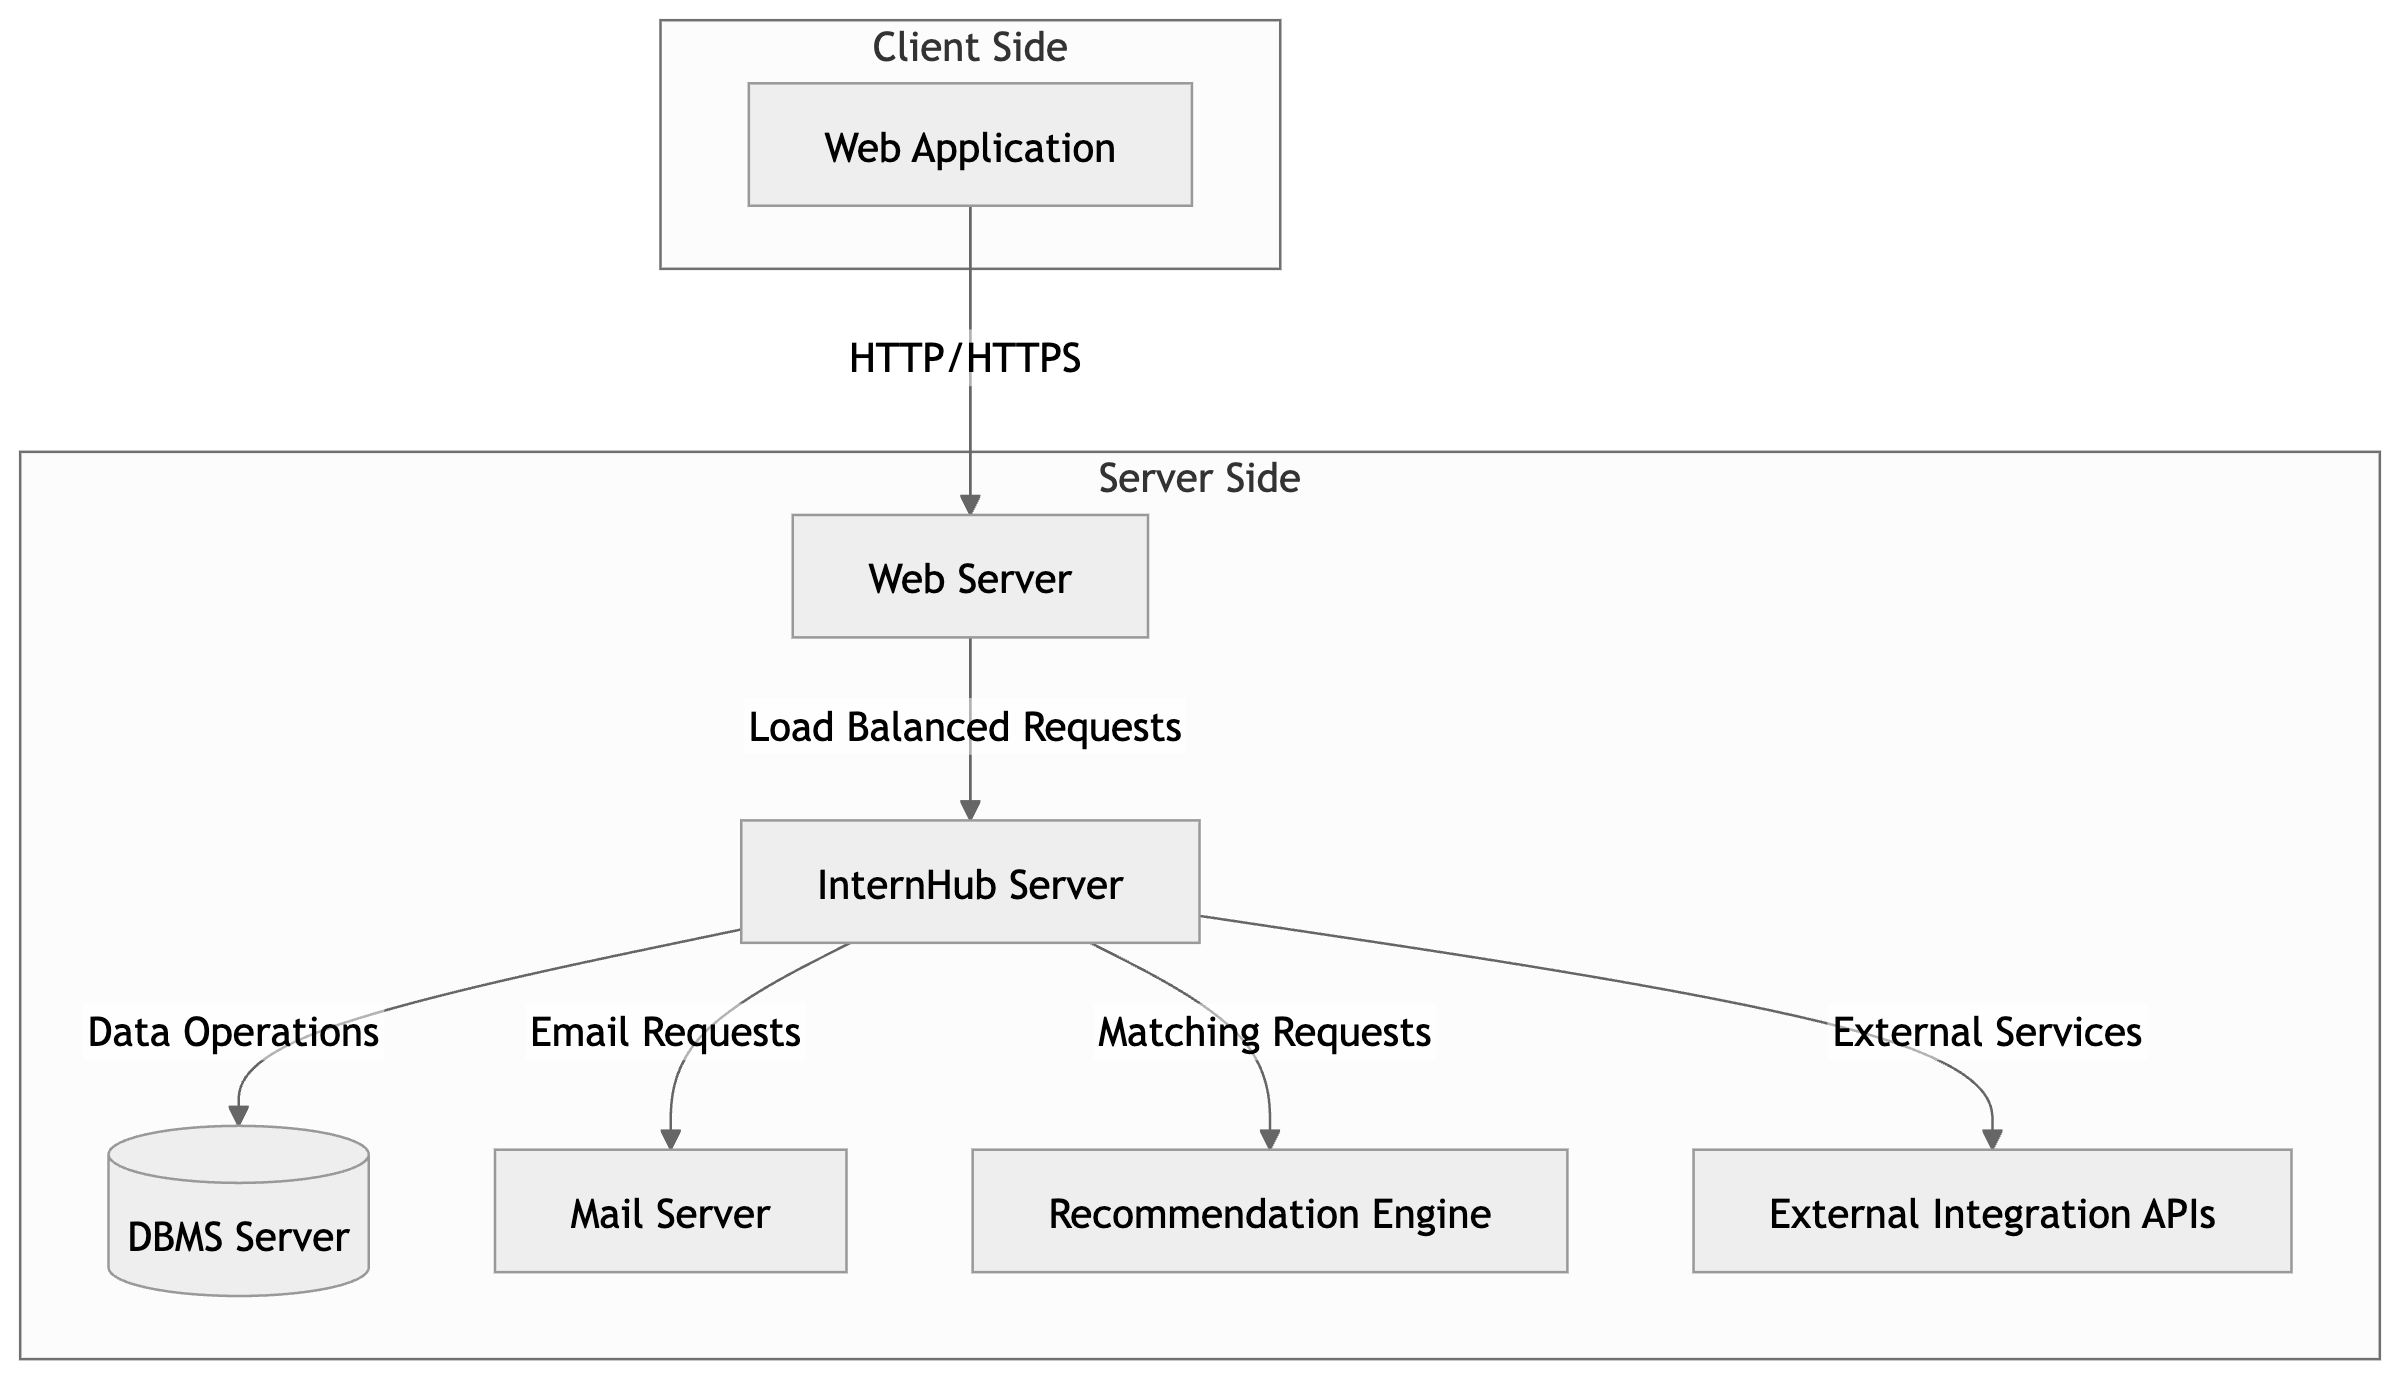
\includegraphics[width=0.82\linewidth]{JhaBhatiaSharma/imagesDD/CKB Overview.png}
        \caption{InternHub Overview}
        \label{fig:internHubOverview}%
    \end{center}
\end{figure}


\subsubsection{Client Side}
\begin{itemize}
    \item \textbf{Web Application:} The main user interface is the web application, which makes the platform accessible to all users—students, companies, and university administration. It makes it possible to do things like register, maintain profiles, post and apply for internships, handle complaints, and examine analytics.
\end{itemize}

\subsubsection{Server Side}
\begin{itemize}
    \item \textbf{Web Server:} Carries out user communications, taking in and processing their requests. For incoming requests, it offers load balancing and divides them among several S\&C Server replicas. To guarantee safe access, it also controls user sessions.
    \item \textbf{S\&C Server:} The center of the platform, which houses all of the interactions. It makes it easier for the database, Web Server, and external APIs to communicate with one another. To manage heavy traffic and guarantee availability, the S\&C Server is replicated over several computers.
    \item \textbf{DBMS Server:} Serves as the primary store for user, internship, application, feedback, and complaint data. It facilitates effective data retrieval and storage for all platform features.
    \item \textbf{Mail Server:} Manages email correspondence, including notifications for internships, changes, and user registration confirmation emails. By informing stakeholders, it improves the user experience.
    \item \textbf{Recommendation Engine API:} Uses advanced algorithms to recommend suitable internships to students based on their profiles and preferences, as well as potential candidates to companies.
    \item \textbf{Analytics Engine API:} Enables stakeholders to make data-driven decisions by offering insights and producing reports about internships, applications, and platform usage.
    \item \textbf{External Tools API:} Enables the safe storage and retrieval of internship-related files, including contracts and certificates, by facilitating integration with document management systems and other outside services.
\end{itemize}

\newpage

\section{Component View}
\label{subsec:component_view}

\subsection{High-Level Diagram}
\label{subsubsec:high_level_diagram}

\begin{figure}[H]
    \begin{center}
        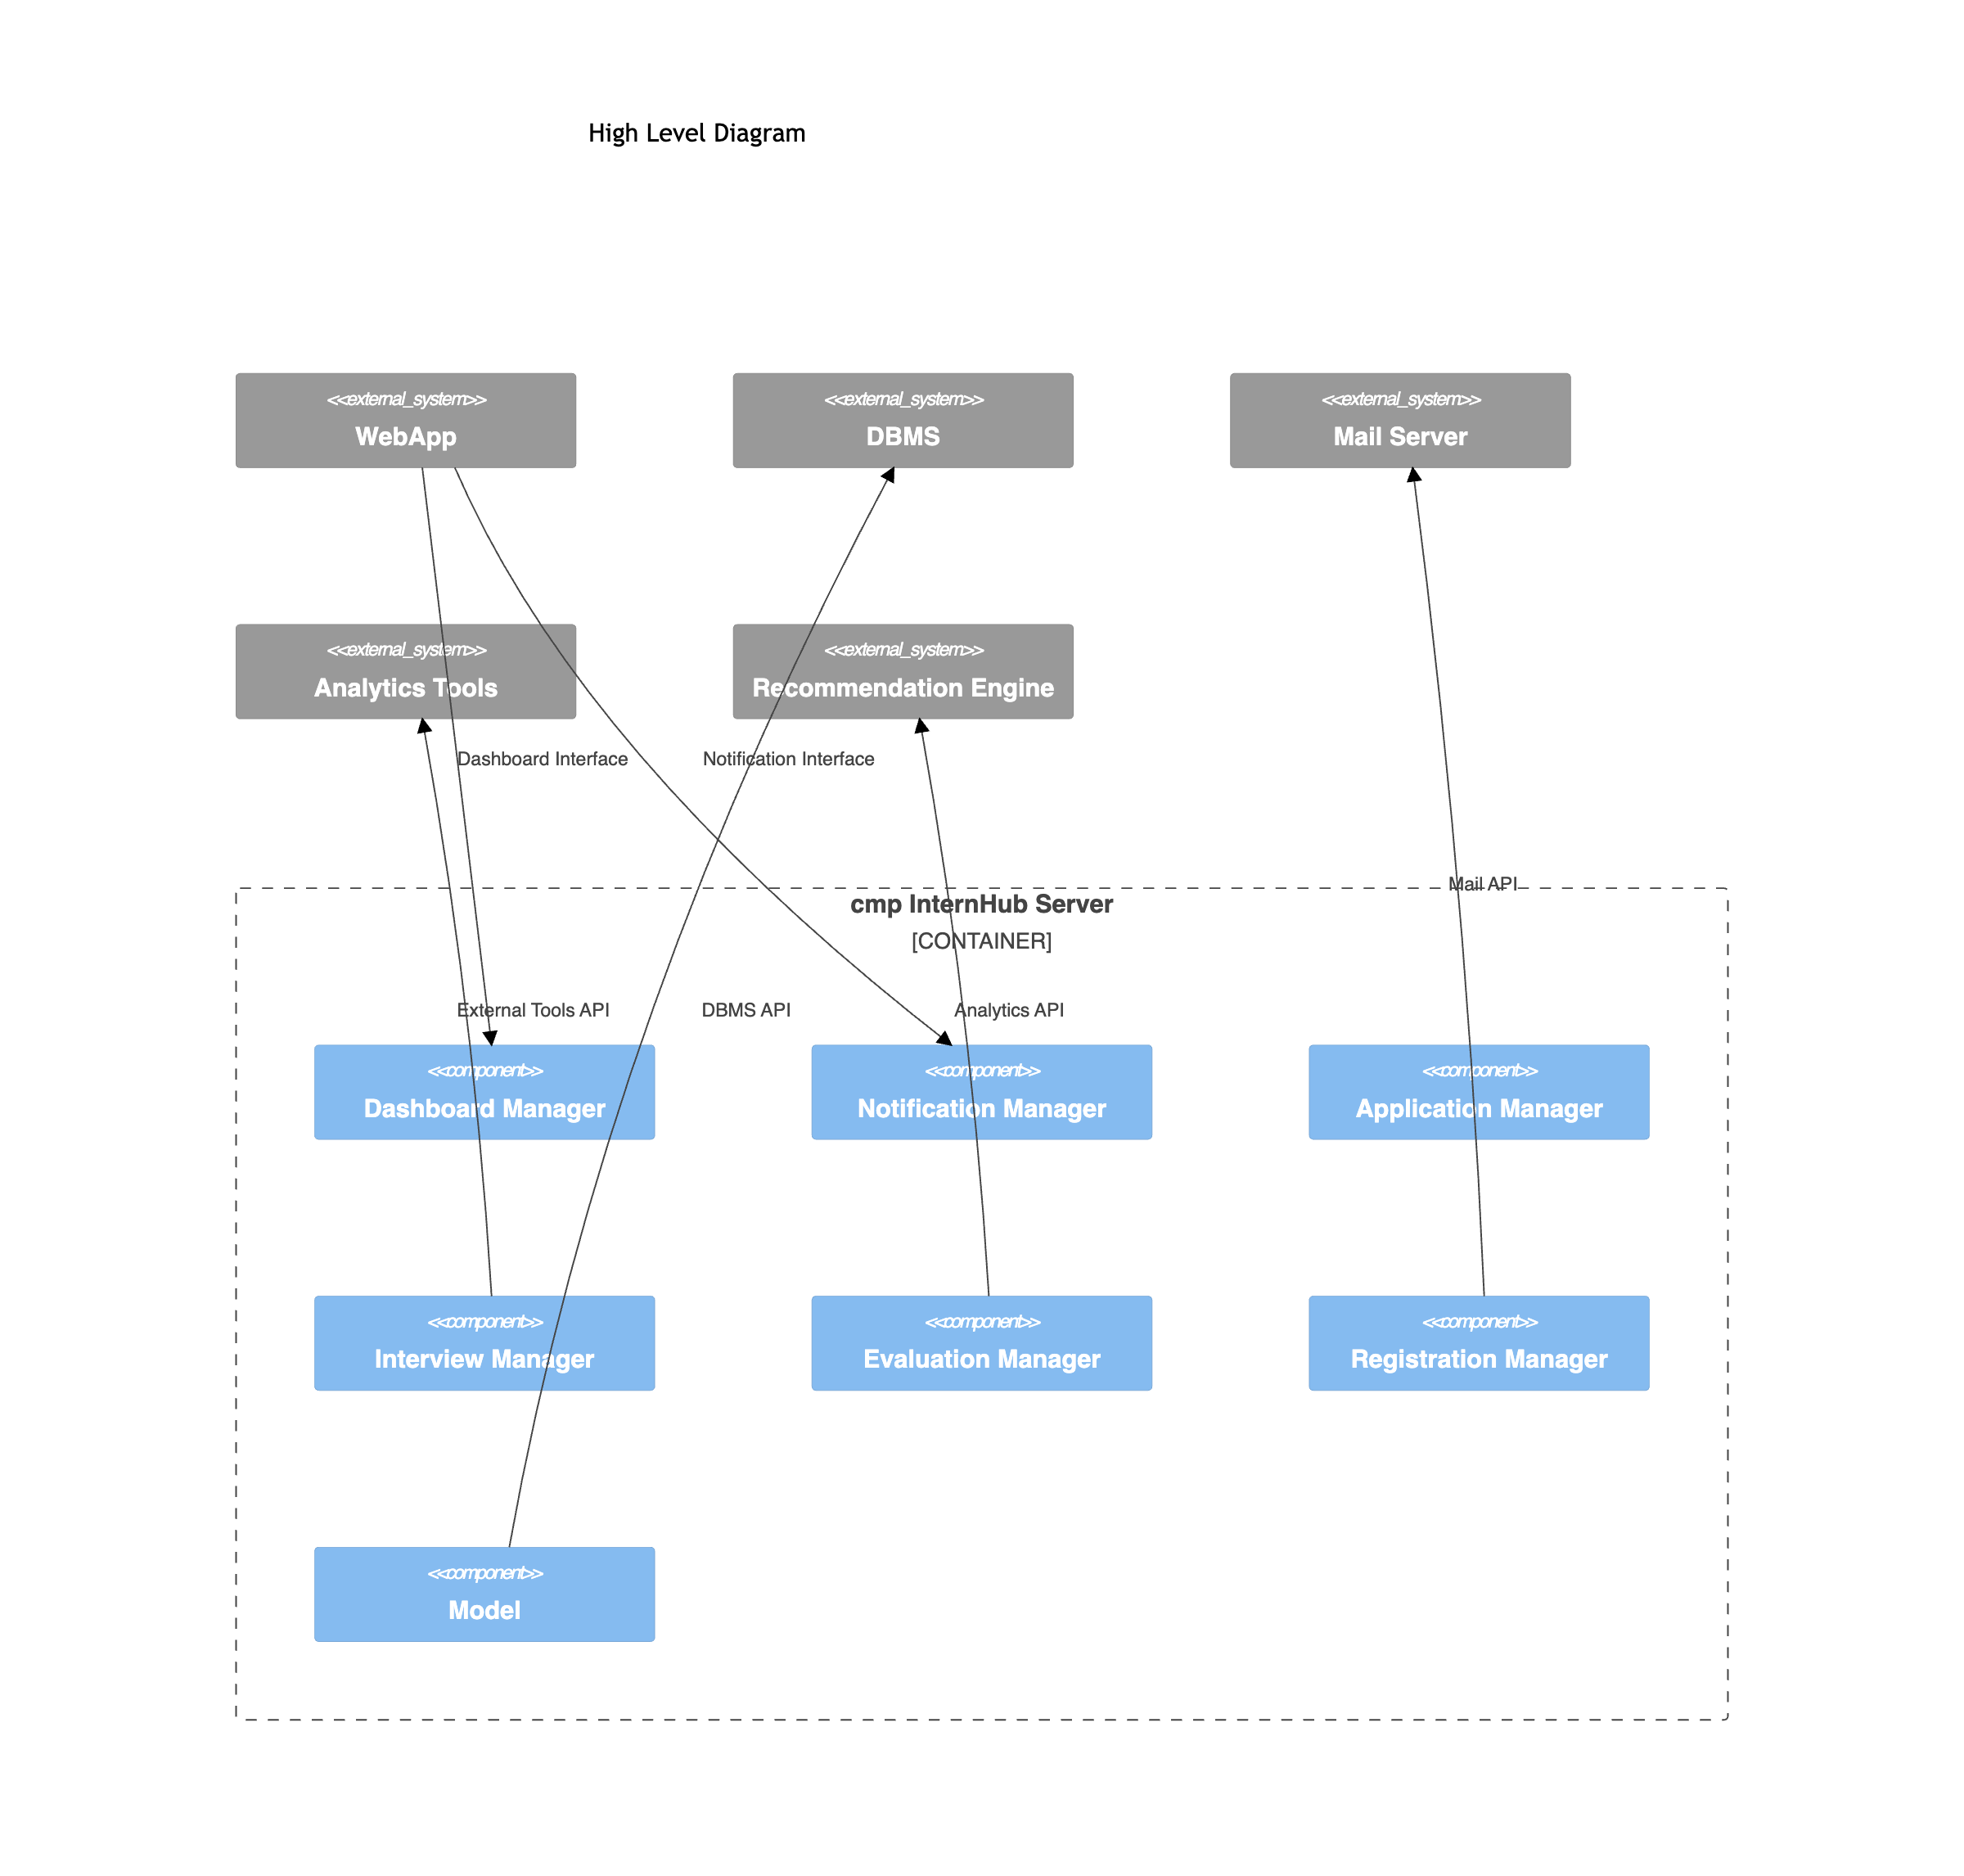
\includegraphics[width=0.82\linewidth]{JhaBhatiaSharma/imagesDD/High Level Diagram.png}
        \caption{High Level Diagram}
        \label{fig:highleveldiagram}%
    \end{center}
\end{figure}

The external components of S\&C are depicted in the high-level component diagram of S\&C above, along with their methods of communication with the S\&C server.

\begin{itemize}
    \item \textbf{WebApp:} Facilitates connectivity with the S\&C Server via the Dashboard Interface, the main channel for client-server communication, by acting as the external access point for users (students, businesses, and university administrators). Through the Notification Interface, the S\&C Server additionally notifies users of updates, reminders, and internship matches.
    \item \textbf{DBMS:} Serves as a storehouse for user profiles, applications, feedback, complaints, and internship posts. Through the DBMS API, which is controlled by the Model Component, it interacts with the S\&C Server.
    \item \textbf{Mail Server:} Manages email correspondence, including alerts for internships and confirmation emails sent after user registration. Through the Mail API, which is connected to the User Registration Manager component, the Mail Server can communicate with the S\&C Server.
    \item
    \textbf{Recommendation Engine:} Employs sophisticated algorithms to suggest internships to prospective employers and students. Through the Recommendation API, which is incorporated into the Matching Engine, it interacts with the S\&C Server.
    \item \textbf{Analytics Engine:} Provides data, analytics, and insights on platform activities, including system utilization, application success rates, and internship patterns. It uses the Analytics API to communicate with the S\&C Server.
    \item \textbf{Document Management System:} Makes it easier to store and retrieve internship-related paperwork securely, including contracts, certifications, and feedback reports. Through the Document Management API, which is incorporated into the File Manager component, it interfaces with the S\&C Server.

    \item \textbf{External System:}
    \begin{itemize}
    \item WebApp connects to the Dashboard Manager and Notification Manager using respective interfaces.
    \item DBMS connects to the Model using the DBMS API.
    \item Mail Server communicates with the Registration Manager through the Mail API.
    \item Recommendation Engine and Analytics Tools interact with the Notification Manager.
    \end{itemize}

    \item \textbf{InternHub Server:}
    The InternHub Server consists of core components like:
\begin{enumerate}
    \item Dashboard Manager
    \item Notification Manager
    \item Application Manager
    \item Registration Manager
    \item Evaluation Manager
    \item Interview Manager
    \item Model for centralized data access
\end{enumerate}
    
\end{itemize}

\subsection{Low-Level Diagram}
\label{subsubsec:low_level_diagram}

\begin{figure}[H]
    \begin{center}
        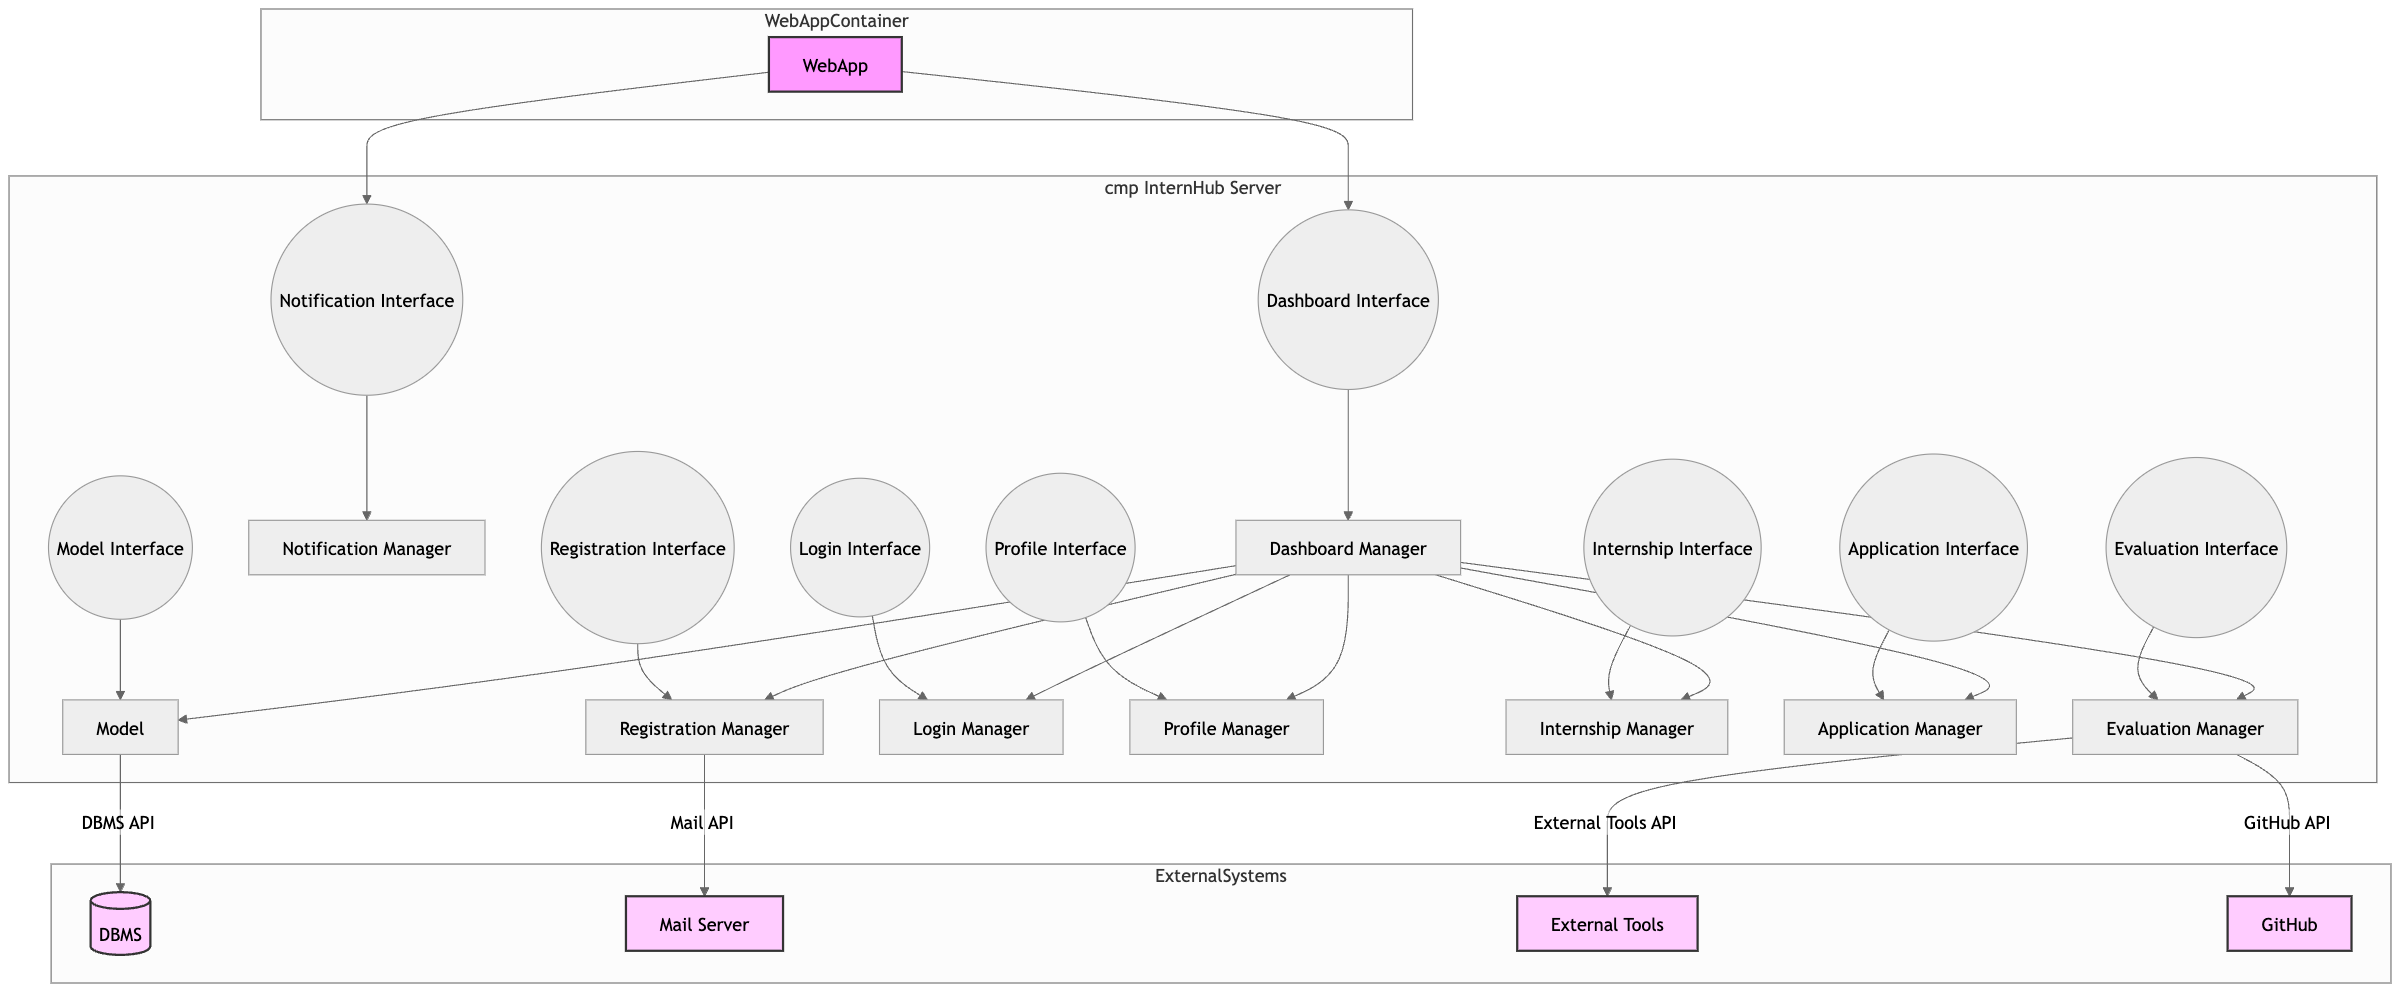
\includegraphics[width=0.82\linewidth]{JhaBhatiaSharma/imagesDD/LowLevelDiagram.png}
        \caption{Low Level Diagram}
        \label{fig:lowleveldiagram}%
    \end{center}
\end{figure}

The figure above represents the detailed architecture of the InternHub – Students \& Companies (S\&C) platform, showing the key components within the InternHub Server and their interactions.

\begin{itemize}
    \item \textbf{Dashboard Manager:} The essential element that plans out all user-platform communication. The Dashboard Manager routes user queries to the appropriate parts of InternHub, while the Dashboard Interface is how users engage with the platform. User activities including managing profiles, looking for internships, and receiving notifications all take place there.

    \item \textbf{Model Component:} Acts as a bridge interface to the DBMS Server and represents the data on the server. It guarantees that all components use the DBMS API to safely and effectively access data.

    \item \textbf{Registration Manager:} Manages the registration of new users, including companies, universities, and students. The Registration Manager handles requests made through the Registration Interface. It interacts with the Model Component to add new user information to the database and with the Mail Server via the Mail API to deliver confirmation emails.

    \item \textbf{Login Manager:} Oversees the registered users' login procedure. The Login Manager handles user login requests sent through the Login Interface. It collects user data from the Model Component and verifies credentials.

    \item \textbf{Profile Manager:} Enables users to search for and browse other users' profiles in addition to managing their own. In order to retrieve or change profile data, the Profile Manager interacts with the Model Component via the Profile Interface.

    \item \textbf{Internship Manager:} Oversees all internship-related activities, such as job advertisements, applications, and status reports.
    \item \textbf{Application Manager:} Manages internship applications, including submission, alerts, and status monitoring. It interacts with the Model Component to retrieve and update data and handles requests through the Application Interface.

    \item \textbf{Evaluation Manager:} Handles the evaluation of students' success during internships.
    \item \textbf{Notification Manager:} In charge of managing every notification that users get. It handles requests through the Notification Interface, including alerting users to platform events, application updates, and internship postings. It interacts with other managers for event triggers and the Model Component for storing notification data.

\end{itemize}

\subsection{Evaluation Manager}
\label{subsubsec:evaluation_manager}
\begin{figure}[H]
    \begin{center}
        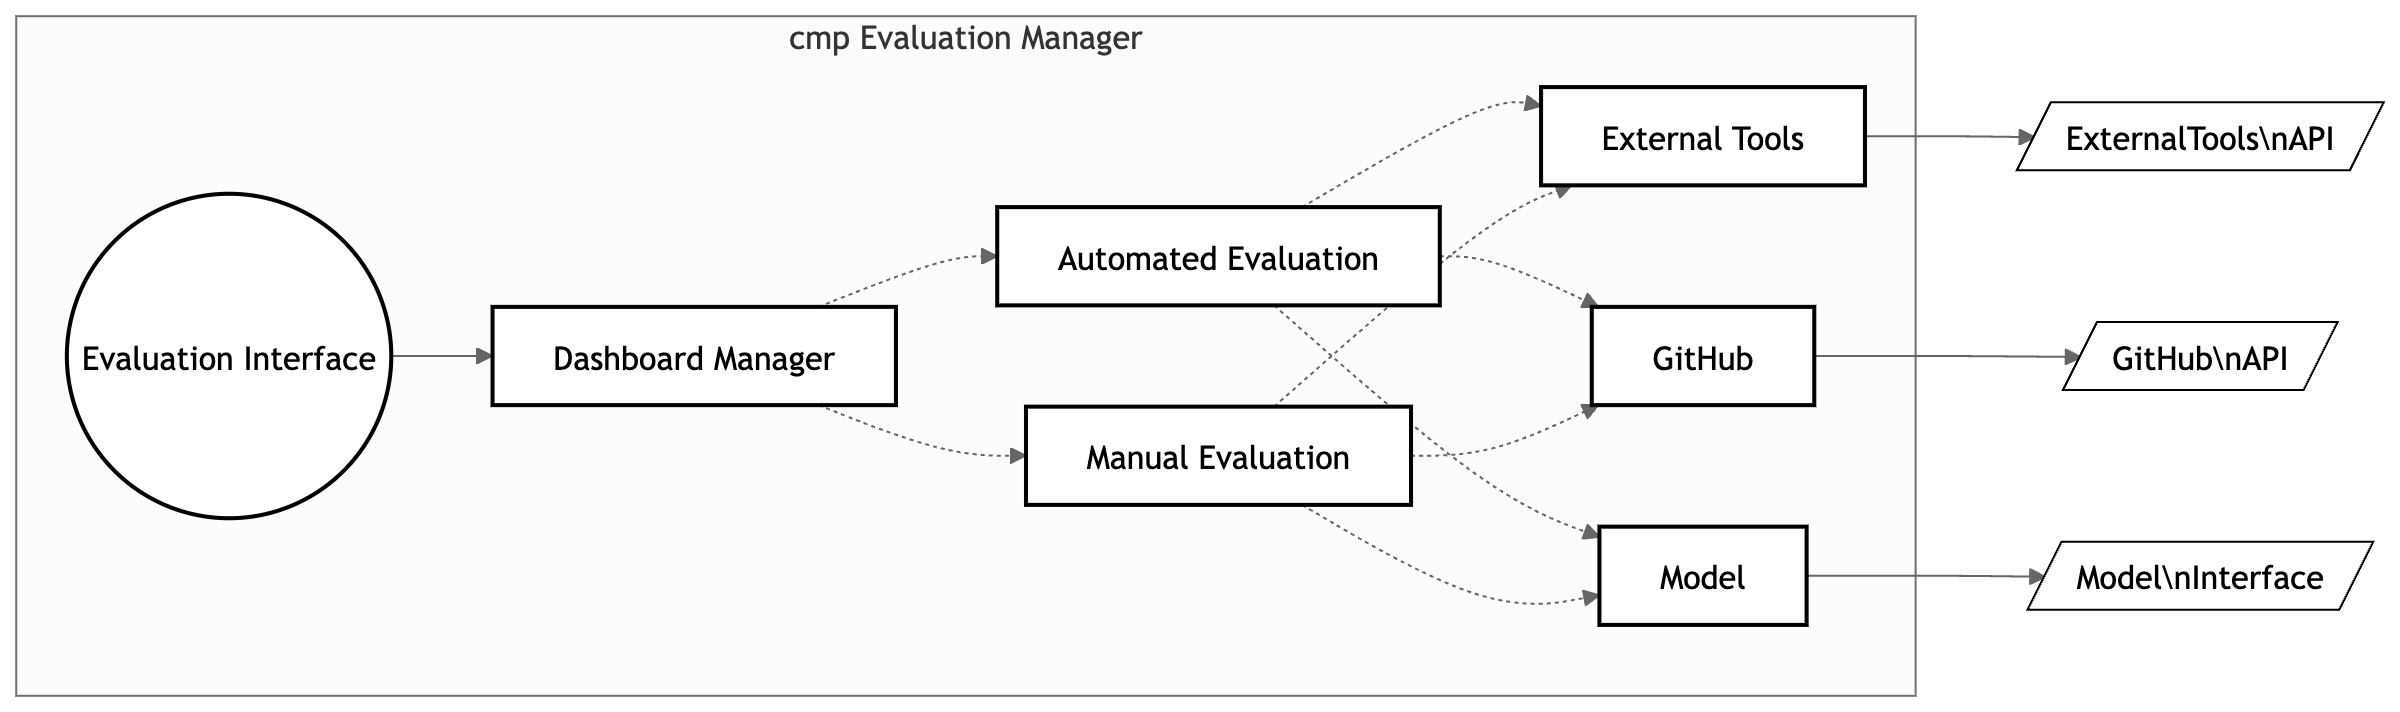
\includegraphics[width=0.82\linewidth]{JhaBhatiaSharma/imagesDD/EvaluationManager.png}
        \caption{Evaluation Manager}
        \label{fig:evaluationmanager}%
    \end{center}
\end{figure}
The InternHub – Students \& Companies (S\&C) platform's Evaluation Manager is designed to evaluate and oversee students' performance reviews during internships. To manage various evaluation techniques, it is divided into two sub-components: Automated Evaluation and Manual Evaluation.

\subsubsection{Automated Evaluation Component}
The Automated Evaluation component is utilized by the InternHub system to automatically assess a student’s performance or task completion during their internship. The workflow is as follows:
\begin{enumerate}
    \item Through the Evaluation Interface, the system notifies the Automated Evaluation Component when an internship milestone or work submission takes place.
    \item Through the External Tools API, the Automated Evaluation component forwards the submitted work to outside tools for evaluation, testing, or scoring (e.g., project testing or task completion verification).
    \item The Automated Evaluation component uses the Model Interface to communicate with the Model Component after receiving the evaluation results from the external tools.
    \item In turn, the Model Component uses the DBMS API to update the student's score in the database, guaranteeing that the evaluation results are appropriately recorded in the appropriate database area.
\end{enumerate}

\subsubsection{Manual Evaluation Component}
The Manual Evaluation component allows companies or university administrators to manually assess a student’s performance during their internship. The process is as follows:
\begin{enumerate}
    \item The evaluator (company or administrator) initiates a request via the WebApp, which connects to the Dashboard Interface.
    \item Through the Evaluation Interface, the request is sent to the Manual Evaluation Component.
    \item The GitHub API or other integrated technologies are used by the Manual Evaluation component to retrieve the student's submitted work or internship data.
    \item The Manual Evaluation component uses the Model Interface to provide the updated results to the Model Component following the evaluator's manual analysis and scoring.
    \item The Model Component ensures that the outcomes of the manual evaluation are accurately documented by updating the scores or evaluations in the database using the DBMS API.
\end{enumerate}

\subsection{Dashboard Manager}
\label{subsubsec:dashboard_manager}

\begin{figure}[H]
    \begin{center}
        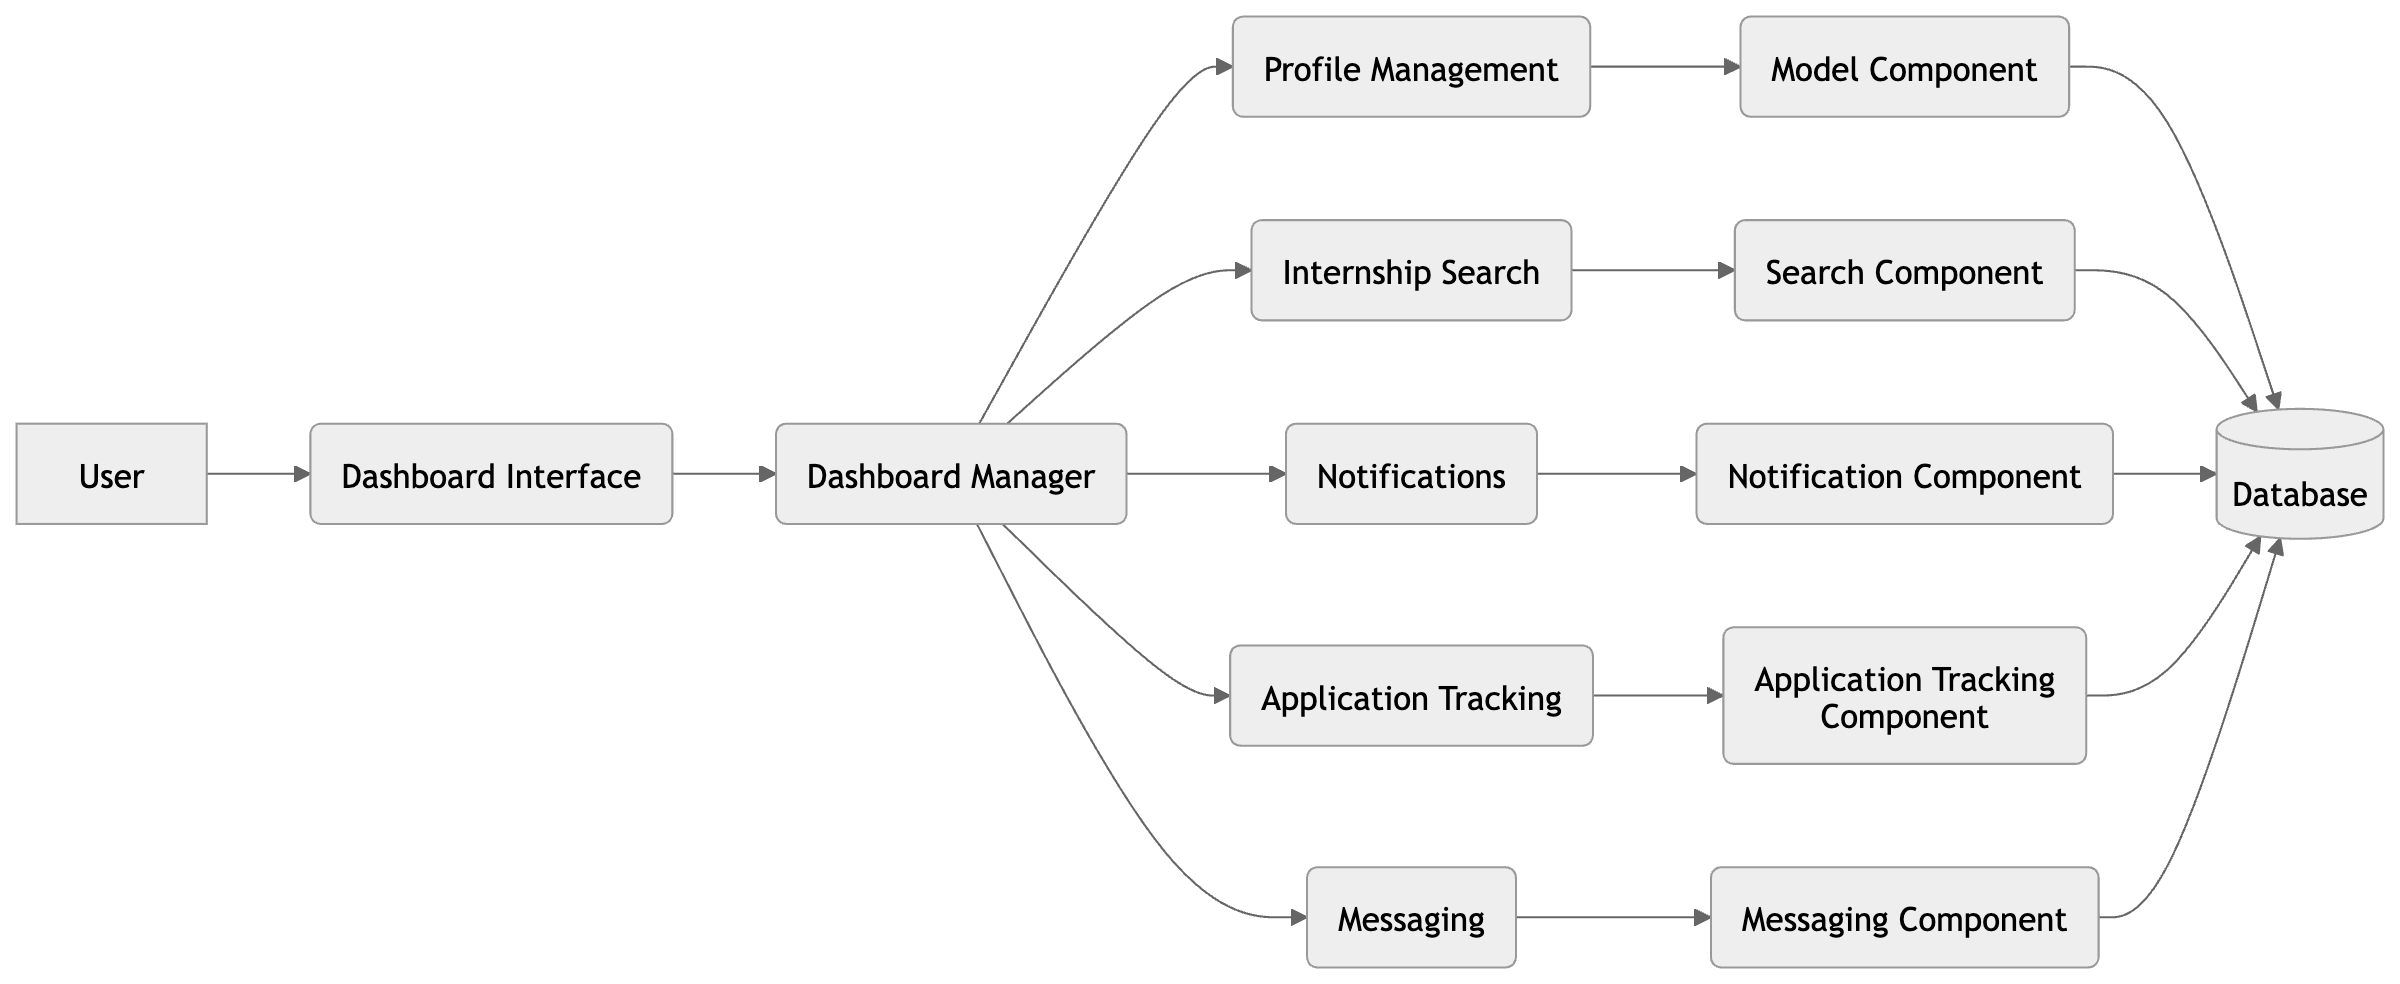
\includegraphics[width=0.82\linewidth]{JhaBhatiaSharma/imagesDD/DashboardManager.png}
        \caption{Dashboard Manager}
        \label{fig:dashboardmanager}%
    \end{center}
\end{figure}

The Dashboard Manager is a pivotal component in the InternHub – Students \& Companies (S\&C) platform, managing user interactions and orchestrating communication between various subsystems. The following outlines its subcomponents and their interactions:

\paragraph{Profile Management}
Users can manage and update their profiles, which include contact details, preferences, and resumes.
\begin{itemize}
    \item In order to retrieve or change user data, the Model Component communicates with the Database and receives requests pertaining to profile management.
\end{itemize}

\paragraph{Internship Search}
Allows users to search and filter internships based on location, preferences, and skills.
\begin{itemize}
    \item These requests are handled by the Search Component, which queries the database and provides users with pertinent results through the Dashboard Interface.
\end{itemize}

\paragraph{Notifications}
Oversees the distribution of user notifications, including critical system messages, profile recommendations, and updates to internship applications.
\begin{itemize}
    \item Interacts with the Notification Component, which provides notification logs and status updates to the database.
\end{itemize}

\paragraph{Application Tracking}
Allows users to keep track of the acceptance, rejection, and company updates on their internship applications.
\begin{itemize}
    \itemIn order to retrieve and present current application statuses, the Application Tracking Component communicates with the database.
\end{itemize}

\paragraph{Messaging}
Facilitates direct communication between administration, businesses, and students to address questions or discuss internships.
\begin{itemize}
    \item Communicates with the Messaging Component, which guarantees that every conversation is recorded and safely kept in the database.
\end{itemize}

\subsection{Profile Manager}
\label{subsubsec:profile_manager}

\begin{figure}[H]
    \begin{center}
        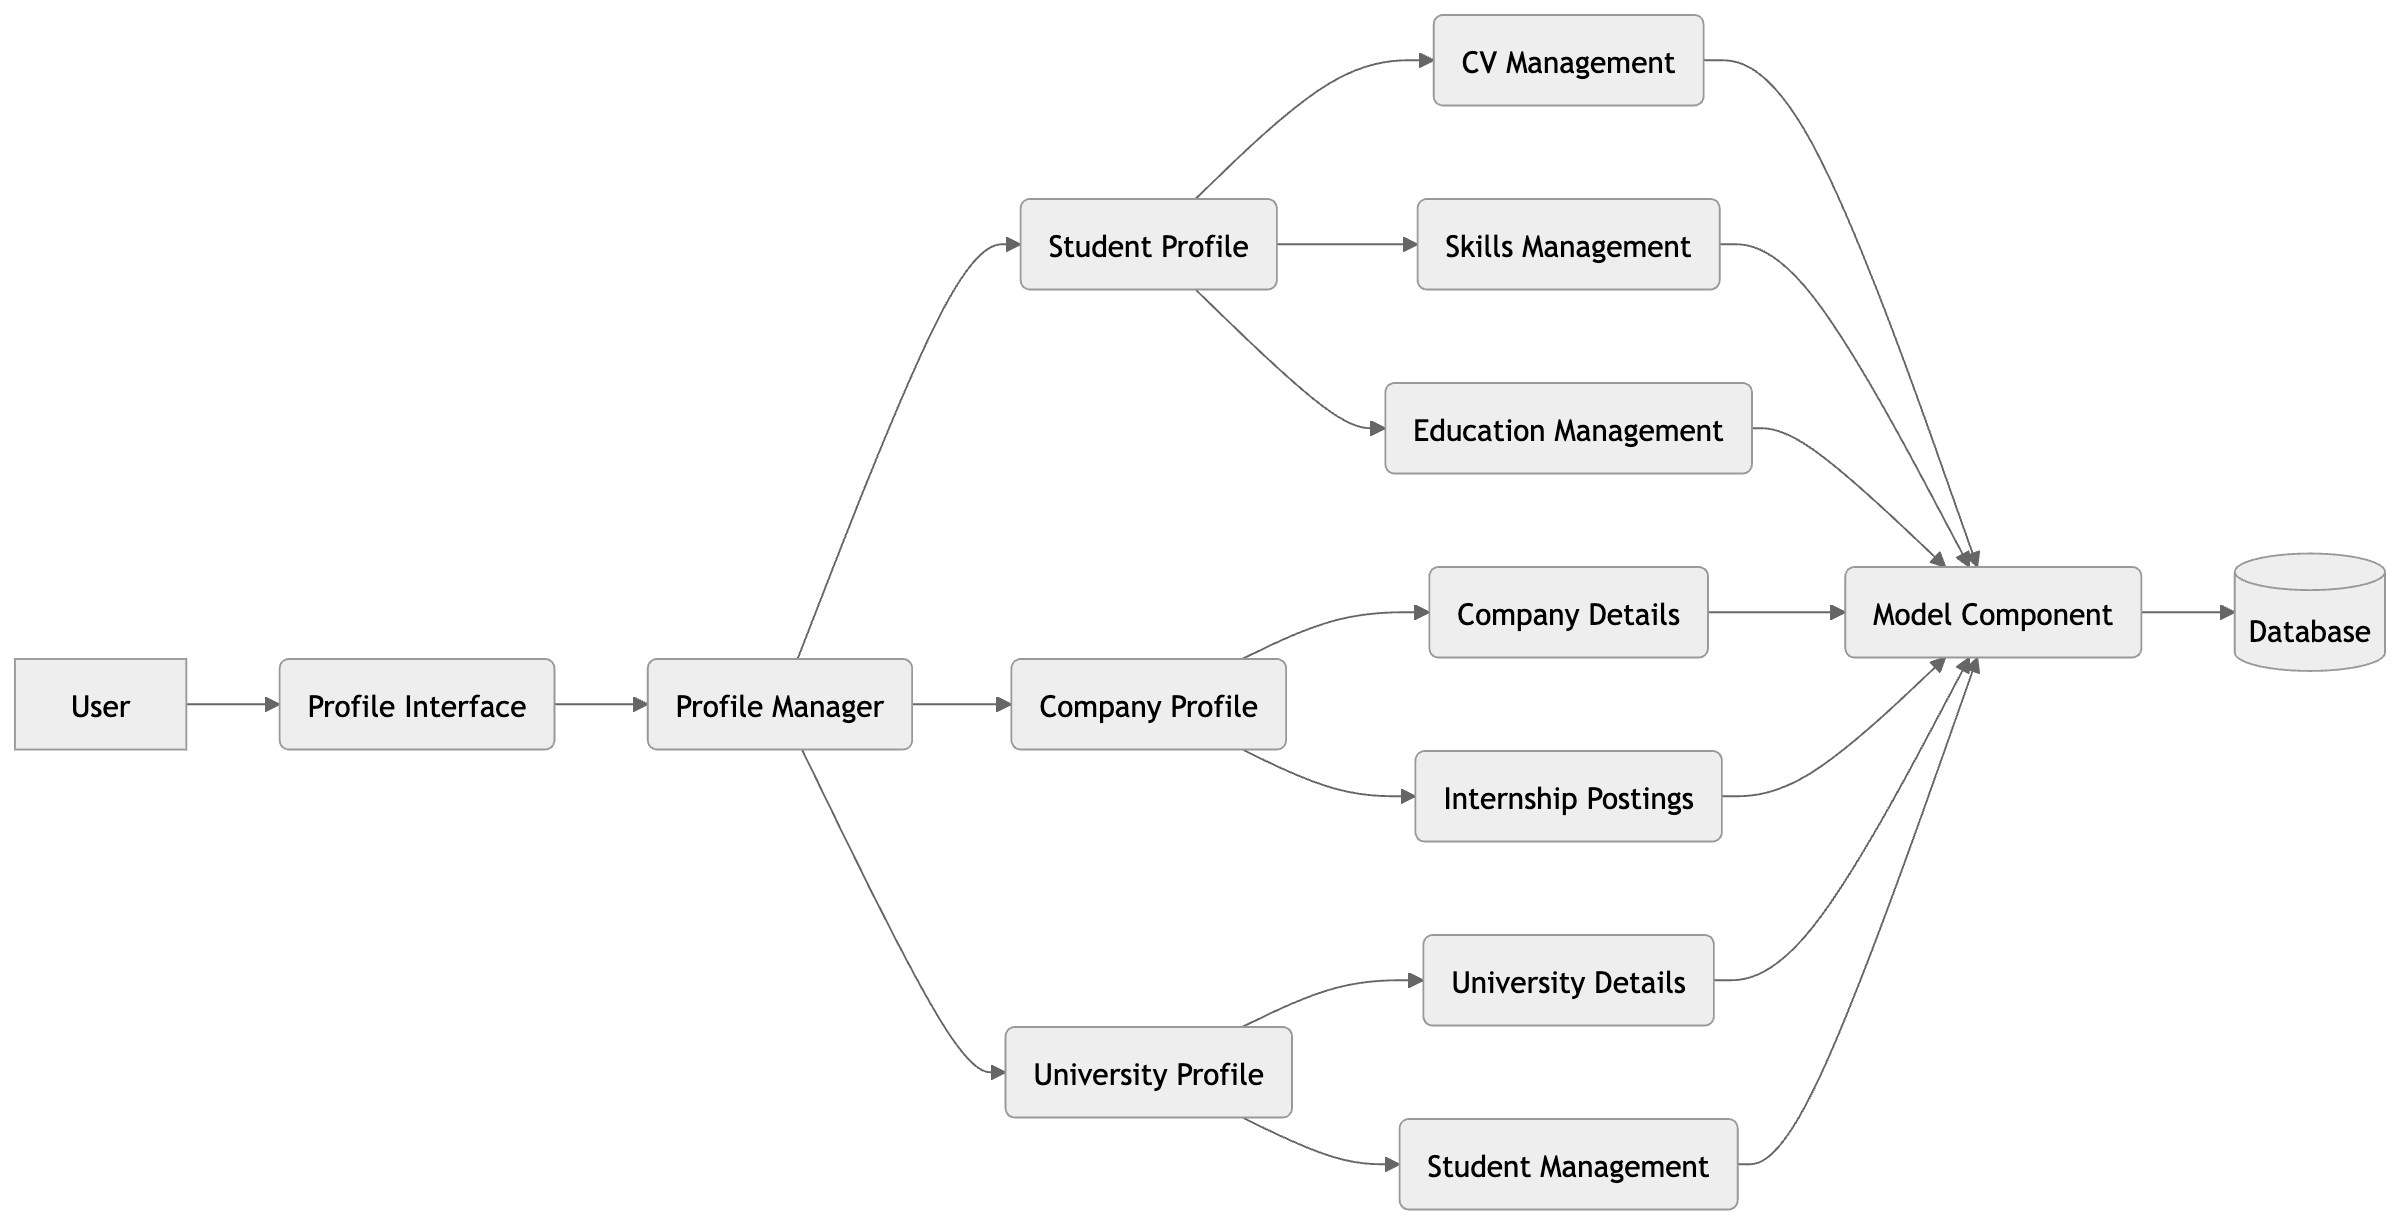
\includegraphics[width=0.82\linewidth]{JhaBhatiaSharma/imagesDD/ProfileManager.png}
        \caption{Profile Manager}
        \label{fig:profilemanager}%
    \end{center}
\end{figure}

The InternHub – Students \& Companies (S\&C) platform's Profile Manager is a key feature that helps institutions, businesses, and students manage and streamline profile-related tasks. To efficiently handle user profile data, the component ensures seamless communication between the Model Component and the database. These are the main subcomponents and their responsibilities:

\paragraph{Student Profile}
Manages student-specific details, including academic achievements, skills, and internship preferences.
\begin{itemize}
    \item \textbf{CV Management:} Handles the creation, modification, and storage of student CVs.
    \item \textbf{Skills Management:} Allows students to add, update, or remove skills based on their expertise.
    \item \textbf{Education Management:} Manages educational history and academic records.
\end{itemize}

\paragraph{Company Profile}
Responsible for maintaining company-related data, such as organizational details, internship postings, and company preferences.
\begin{itemize}
    \item \textbf{Company Details:} Stores and updates company information, such as name, size, industry, and contact details.
    \item \textbf{Internship Postings:} Enables companies to create, modify, and manage internship listings.
\end{itemize}

\paragraph{University Profile}
Oversees university-specific information and ensures administrators have tools to manage student profiles and internships.
\begin{itemize}
    \item \textbf{University Details:} Handles institutional information, including department details and associated staff.
    \item \textbf{Student Management:} Allows universities to monitor and manage student data and progress.
\end{itemize}

\subsection{Internship Manager}
\label{subsec:internship_manager}
\begin{figure}[H]
    \begin{center}
        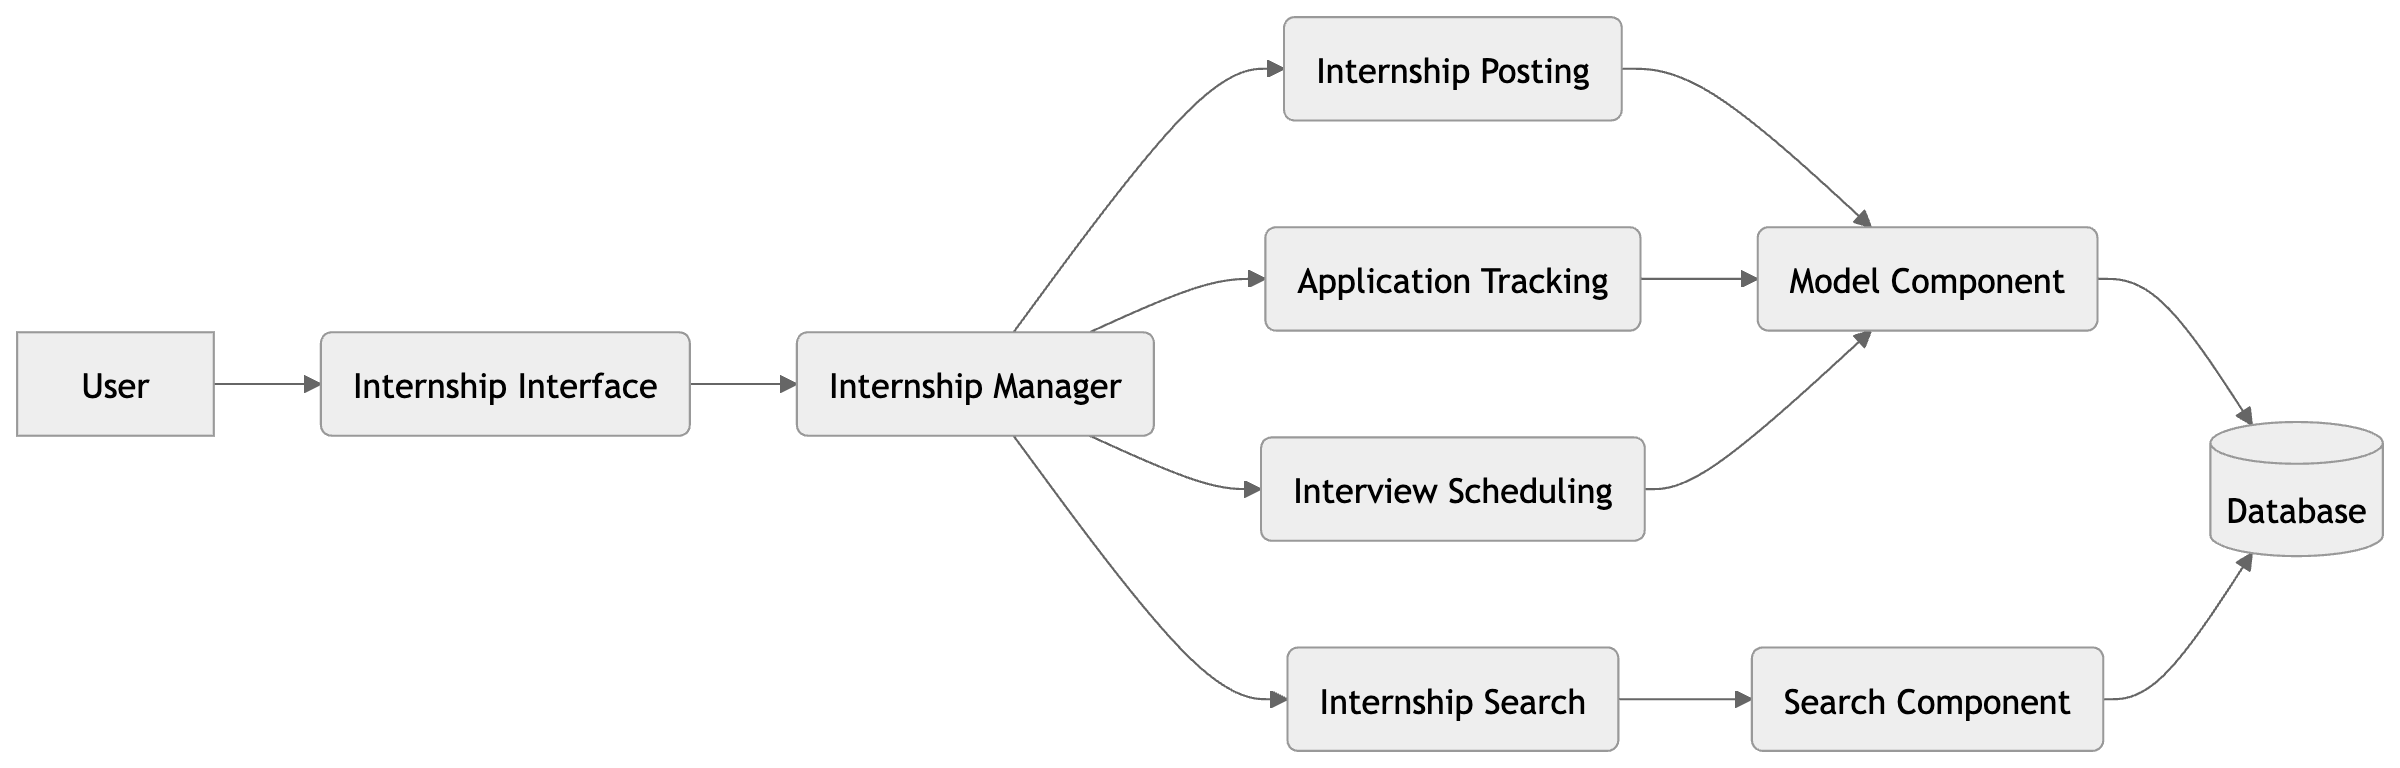
\includegraphics[width=0.82\linewidth]{JhaBhatiaSharma/imagesDD/InternshipManager.png}
        \caption{Internship Manager}
        \label{fig:internshipmanager}%
    \end{center}
\end{figure}

Managing the internship lifecycle is the primary responsibility of the InternHub – Students \& Companies (S\&C) platform's Internship Manager. It facilitates effective handling of internship-related features by managing user interactions with the platform. Below is a summary of its constituents and interrelations:

\paragraph{Internship Posting}
\begin{itemize}
    \item Allows companies to create, update, and manage internship opportunities.
    \item Interacts with the Model Component to store and retrieve data from the Database.
    \item Ensures all postings are accessible to students via the Internship Search feature.
\end{itemize}

\paragraph{Application Tracking}
\begin{itemize}
    \item Enables students and companies to monitor the status of internship applications in real-time.
    \item Communicates with the Model Component to update and retrieve application details from the Database.
    \item Provides notifications to users regarding application progress or results.
\end{itemize}

\paragraph{Interview Scheduling}
\begin{itemize}
    \item Handles the scheduling of interviews between students and companies as part of the internship process.
    \item Retrieves and updates scheduling data in the Database through the Model Component.
\end{itemize}

\paragraph{Internship Search}
\begin{itemize}
    \item Helps students search for internships based on criteria such as location, skills, or duration.
    \item Uses the Search Component to query the Database and fetch matching results.
    \item Provides personalized recommendations based on student profiles and preferences.
\end{itemize}

\subsection{Application Manager}
\label{subsec:application_manager}
\begin{figure}[H]
    \begin{center}
        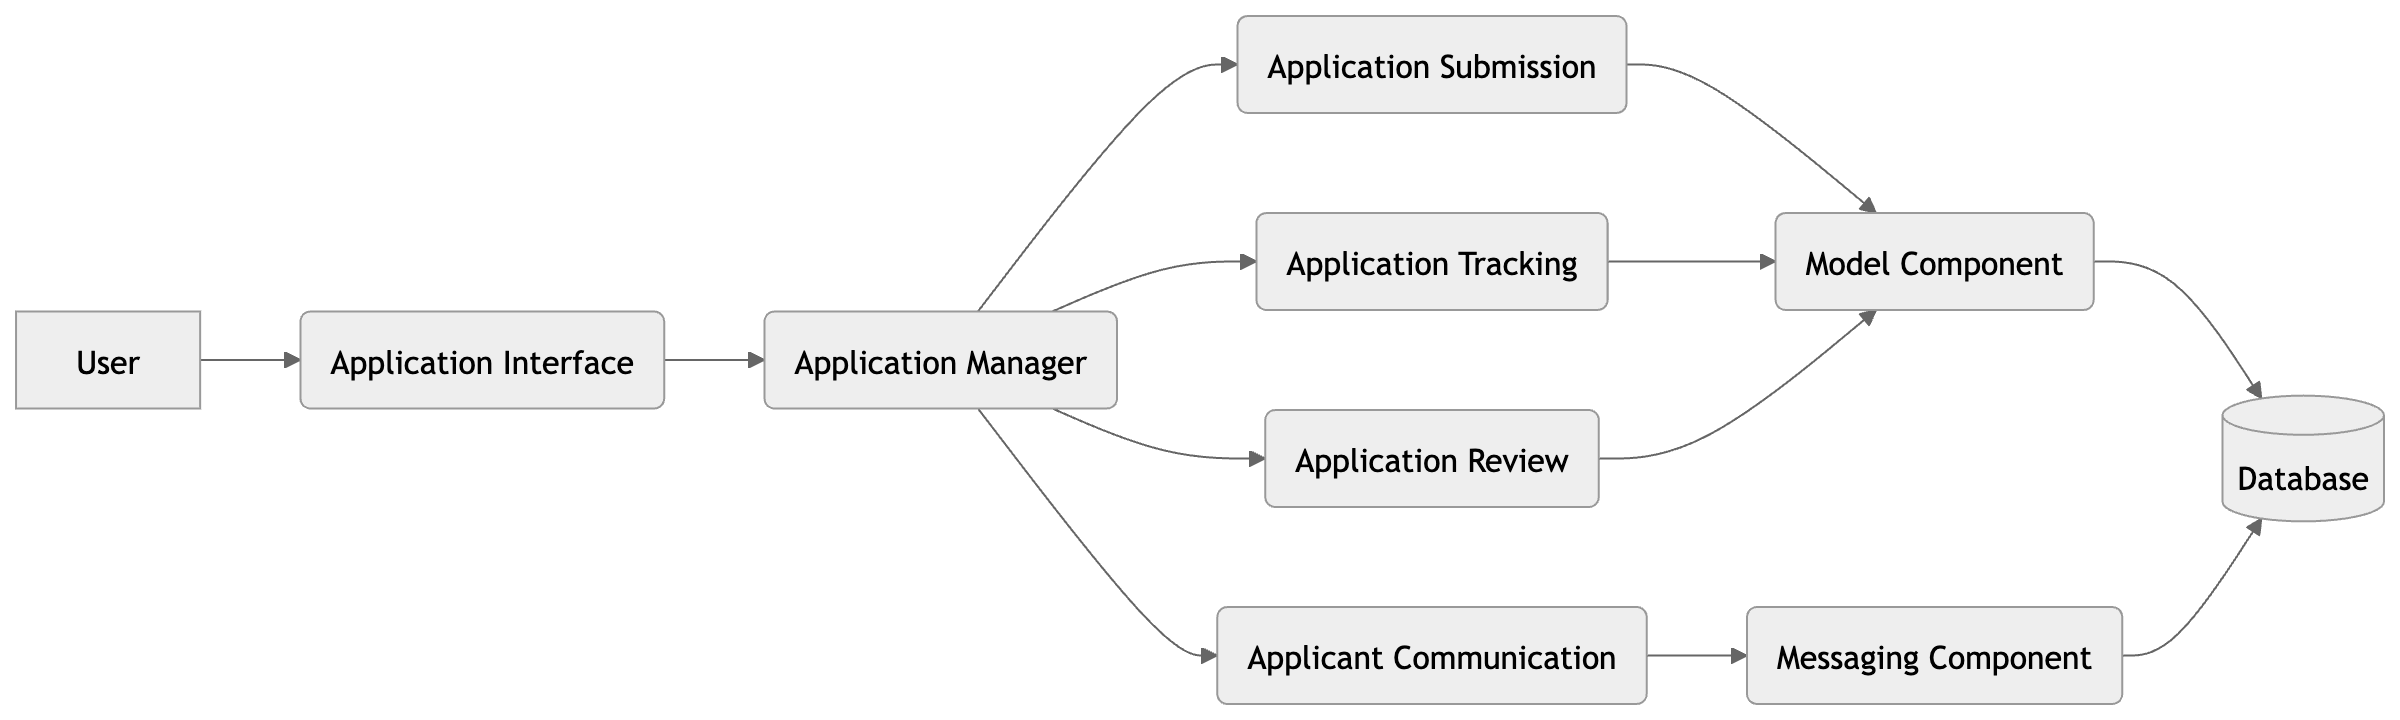
\includegraphics[width=0.82\linewidth]{JhaBhatiaSharma/imagesDD/ApplicationManager.png}
        \caption{Application Manager}
        \label{fig:applicationmanager}%
    \end{center}
\end{figure}

The Application Manager is responsible for handling all operations related to internship applications, ensuring seamless interaction between students, companies, and the platform.

\paragraph{Application Submission}
\begin{itemize}
    \item Manages the submission of internship applications by students.
    \item Interacts with the Model Component to store the application data in the Database.
\end{itemize}

\paragraph{Application Tracking}
\begin{itemize}
    \item Allows students and companies to monitor the status of submitted applications.
    \item Communicates with the Model Component to retrieve and update application status in the Database.
\end{itemize}

\paragraph{Application Review}
\begin{itemize}
    \item Enables companies to review applications submitted by students.
    \item Retrieves application details from the Model Component and updates the status post-review in the Database.
\end{itemize}

\paragraph{Applicant Communication}
\begin{itemize}
    \item Facilitates direct communication between applicants and companies regarding applications.
    \item Utilizes the Messaging Component to send and receive messages, with all interactions logged in the Database.
\end{itemize}

\section{Deployment View}
\label{sec:deployment_view}

\begin{figure}[H]
    \begin{center}
        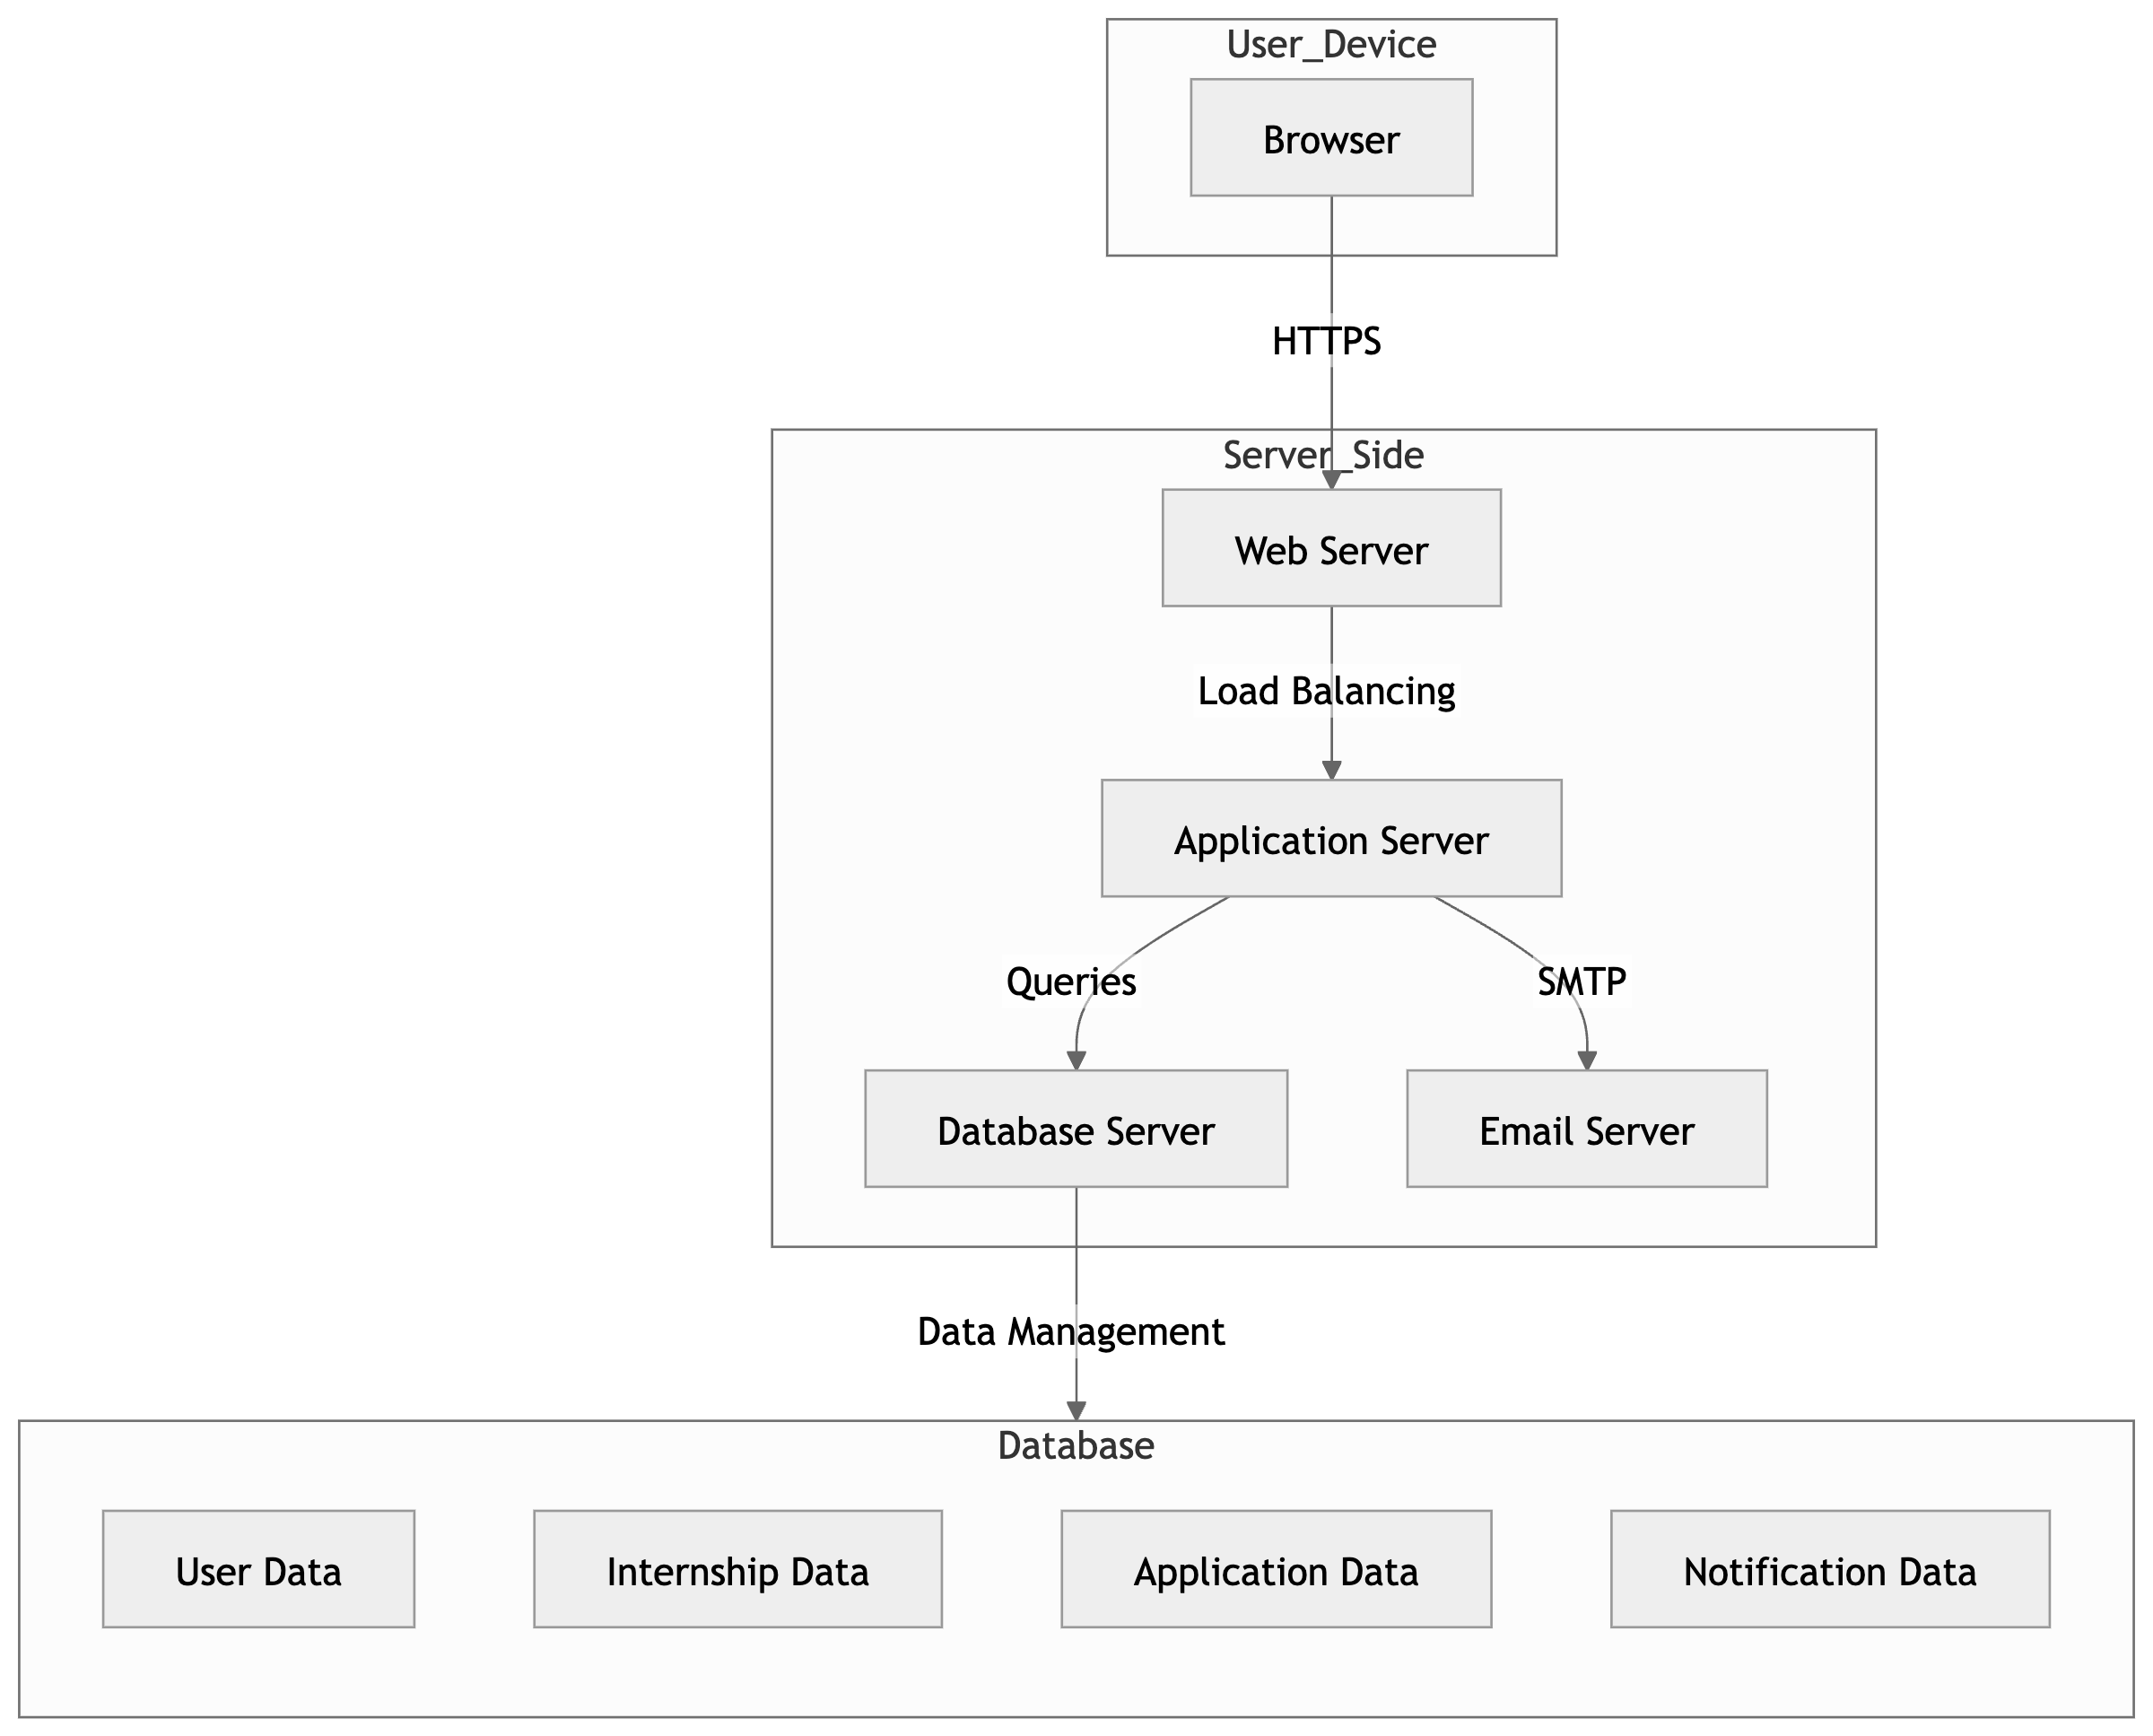
\includegraphics[width=0.82\linewidth]{JhaBhatiaSharma/imagesDD/DeploymentView.png}
        \caption{Deployment View}
        \label{fig:deploymentview}%
    \end{center}
\end{figure}
The platform's deployment architecture is composed of the following layers:

\paragraph{Client Side}
\begin{itemize}
    \item User devices, which are mostly accessed through web browsers, make up the client side. These devices stand in for platform users, which include companies, educational institutions, and students.
    \item Users engage with platform services such as applications, notifications, internship posts, profile management, registration, and login using their browsers.
    \item HTTPS ensures data privacy and protection by securing communication between the user and the platform.
\end{itemize}

\paragraph{Server Side}
\begin{itemize}
    \item \textbf{Web Server:} serves as the gateway for all requests from clients. By allocating incoming requests to several application server replicas, it performs load balancing, guarantees secure HTTPS connections, and controls the delivery of static content (HTML, CSS, and JavaScript).
    \item \textbf{Application Server:} acts as the main backend, coordinating with other parts and processing business logic. Notification delivery, internship management, and user management are all handled by it. For data storage and retrieval, it interfaces with the DBMS Server; for automated communication, it integrates with the Email Server.
    \item \textbf{DBMS Server:} keeps application, user, and internship-related data. Notifications are recorded, and effective data updates, retrieval, and storage are guaranteed.
    \item \textbf{Email Server:} uses the SMTP protocol to handle outward messages, including application updates and registration confirmations.
\end{itemize}

\section{Runtime View}
\label{sec:runtime_view}

\subsection{Sign-Up Process}
\label{subsec:signup_process}
\begin{figure}[H]
    \begin{center}
        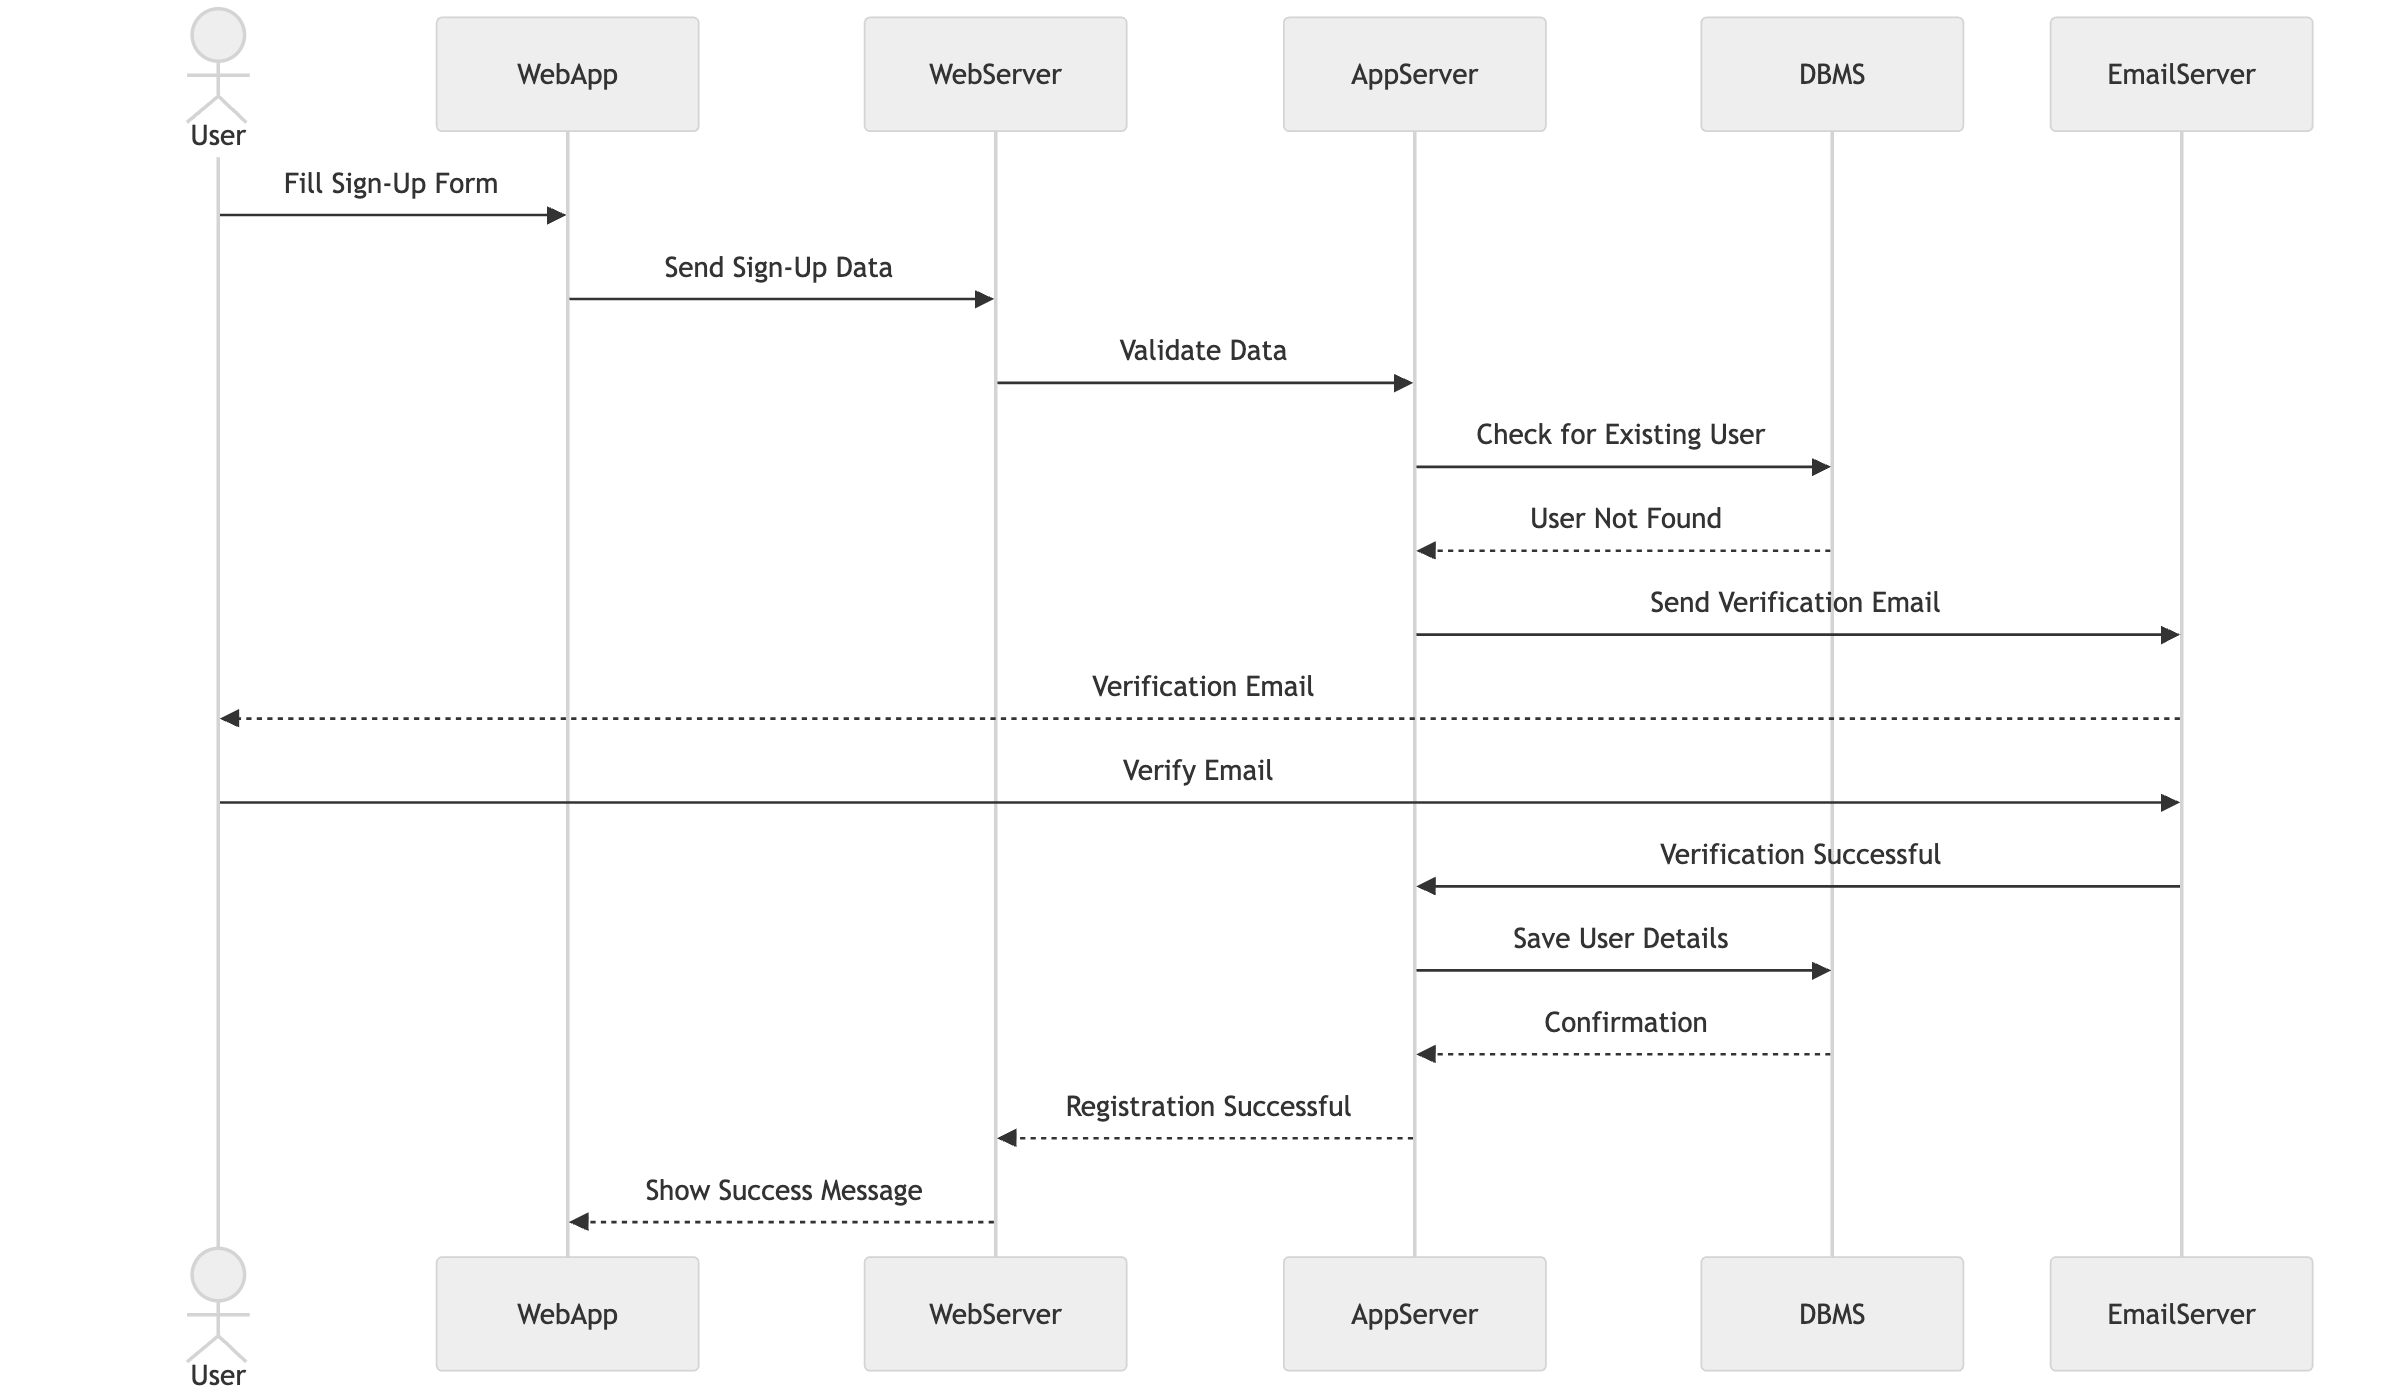
\includegraphics[width=0.82\linewidth]{JhaBhatiaSharma/imagesDD/SignUpRuntime.png}
        \caption{Runtime SignUp}
        \label{fig:signupruntime}%
    \end{center}
\end{figure}

The platform's sign-up process allows new users (students, companies, or university administrators) to register. The process is as follows:
\begin{enumerate}
    \item Through the WebApp's sign-up form, the user provides their name, email address, password, and user role.
    \item After confirming the inputs, the Web Server securely sends the data to the Application Server.
    \item The DBMS Server is used by the Application Server's Registration Manager component to search the database for duplicate records.
    \item The Email Server sends a verification email if the user is unique.
    \item The Application Server validates successful registration and saves the user's information in the database after confirming the email.
\end{enumerate}

\subsection{Login Process}
\label{subsec:login_process}

\begin{figure}[H]
    \begin{center}
        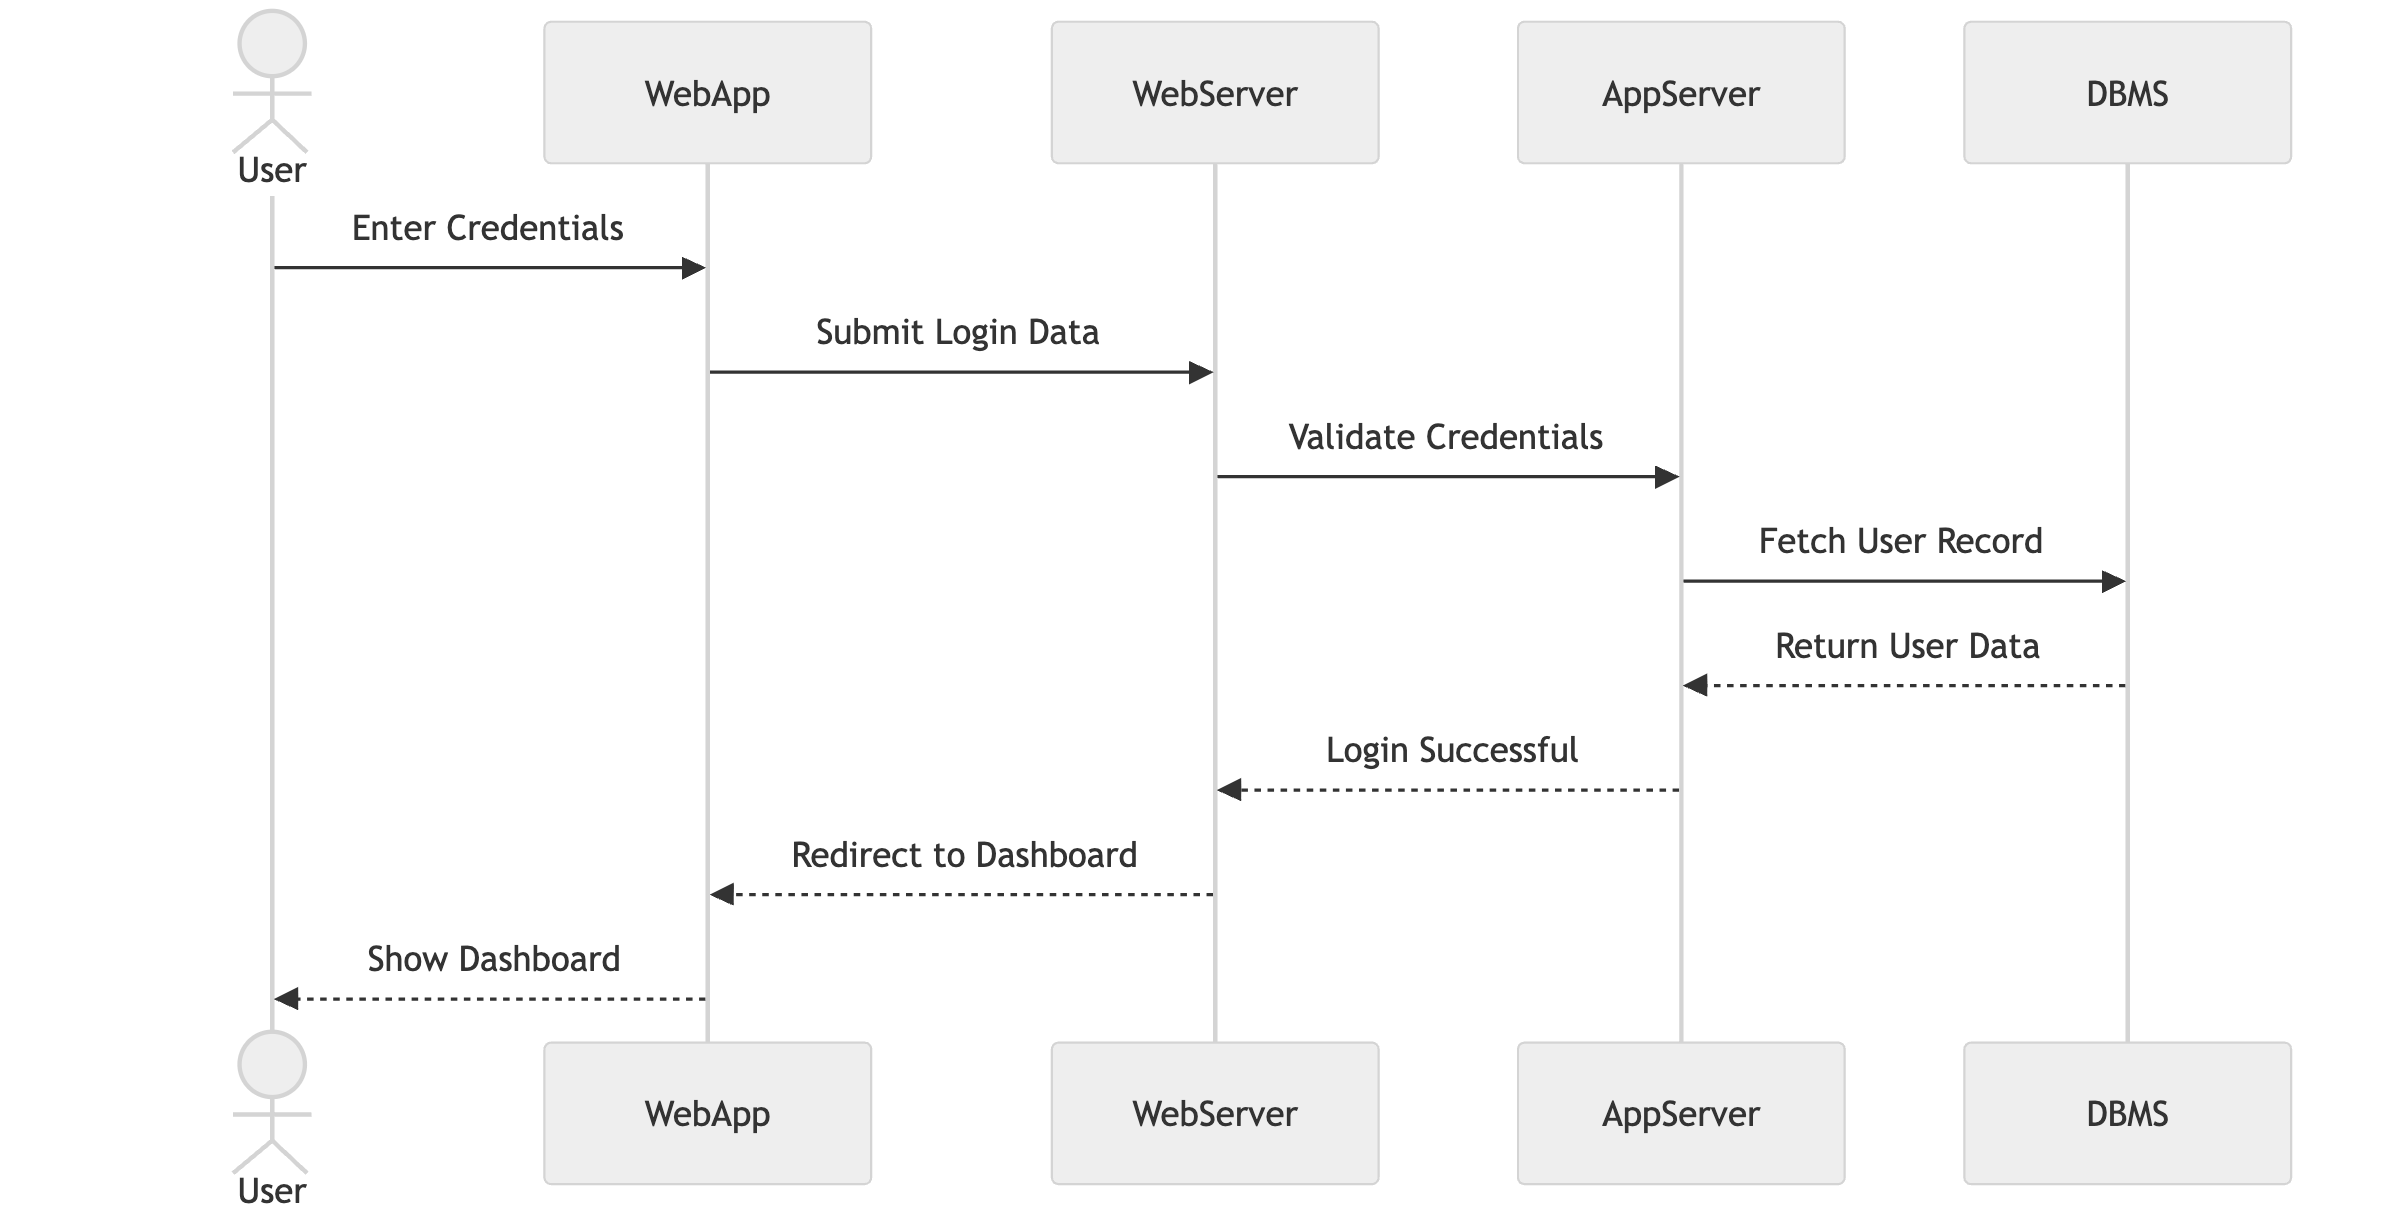
\includegraphics[width=0.82\linewidth]{JhaBhatiaSharma/imagesDD/LoginRuntime.png}
        \caption{Runtime Login}
        \label{fig:loginruntime}%
    \end{center}
\end{figure}

The login process ensures secure access for registered users. The steps are as follows:
\begin{enumerate}
    \item The user inputs their credentials on the WebApp’s login form.
    \item The Application Server receives the data safely from the Web Server.
    \item Through the DBMS Server, the Application Server's Login Manager compares the credentials against database entries.
    \item The system creates a session token and logs the user into the platform if the credentials match.
    \item To ensure easy and safe access, the user is taken to their dashboard.
\end{enumerate}

\subsection{Post Internship}
\label{subsec:post_internship}
\begin{figure}[H]
    \begin{center}
        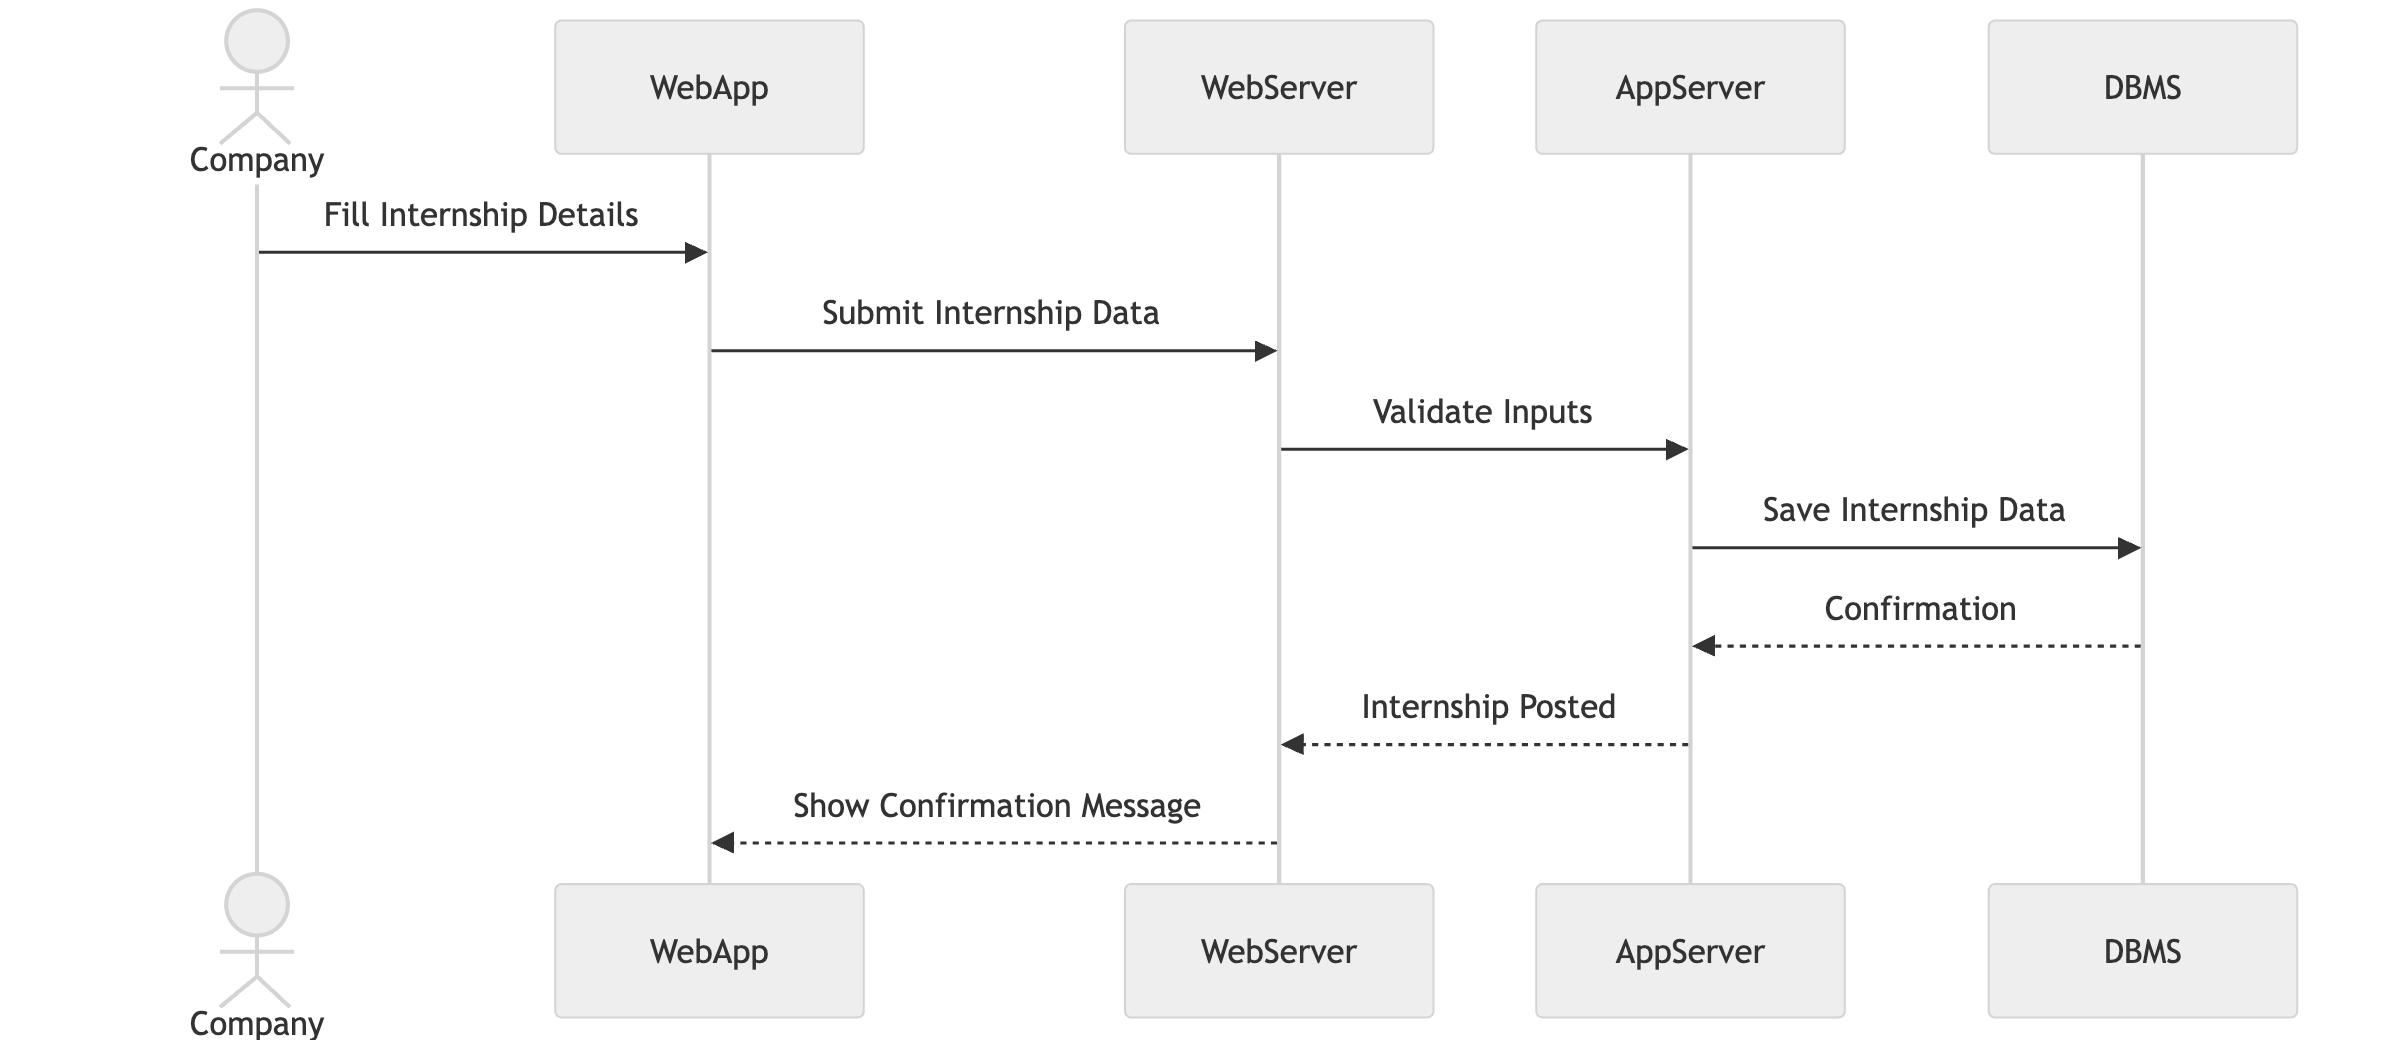
\includegraphics[width=0.82\linewidth]{JhaBhatiaSharma/imagesDD/PostInternshipRuntime.png}
        \caption{Runtime Post Internship}
        \label{fig:postinternshpruntime}%
    \end{center}
\end{figure}
Posting an internship is an essential function for company users. The process is as follows:
\begin{enumerate}
    \item By completing the internship details using the WebApp, including the job title, description, requirements, and duration, the company user starts the process.
    \item After receiving this data, the Web Server sends it to the Application Server for validation.
    \item The new internship posting is stored in the database by the Internship Manager component, which handles data processing and communication with the DBMS Server.
    \item A confirmation message is sent to the company user when the data has been successfully stored.
\end{enumerate}
This process ensures that the posted internship is immediately visible to qualified students looking for opportunities.

\subsection{Interview Management}
\label{subsec:interview_management}
\begin{figure}[H]
    \begin{center}
        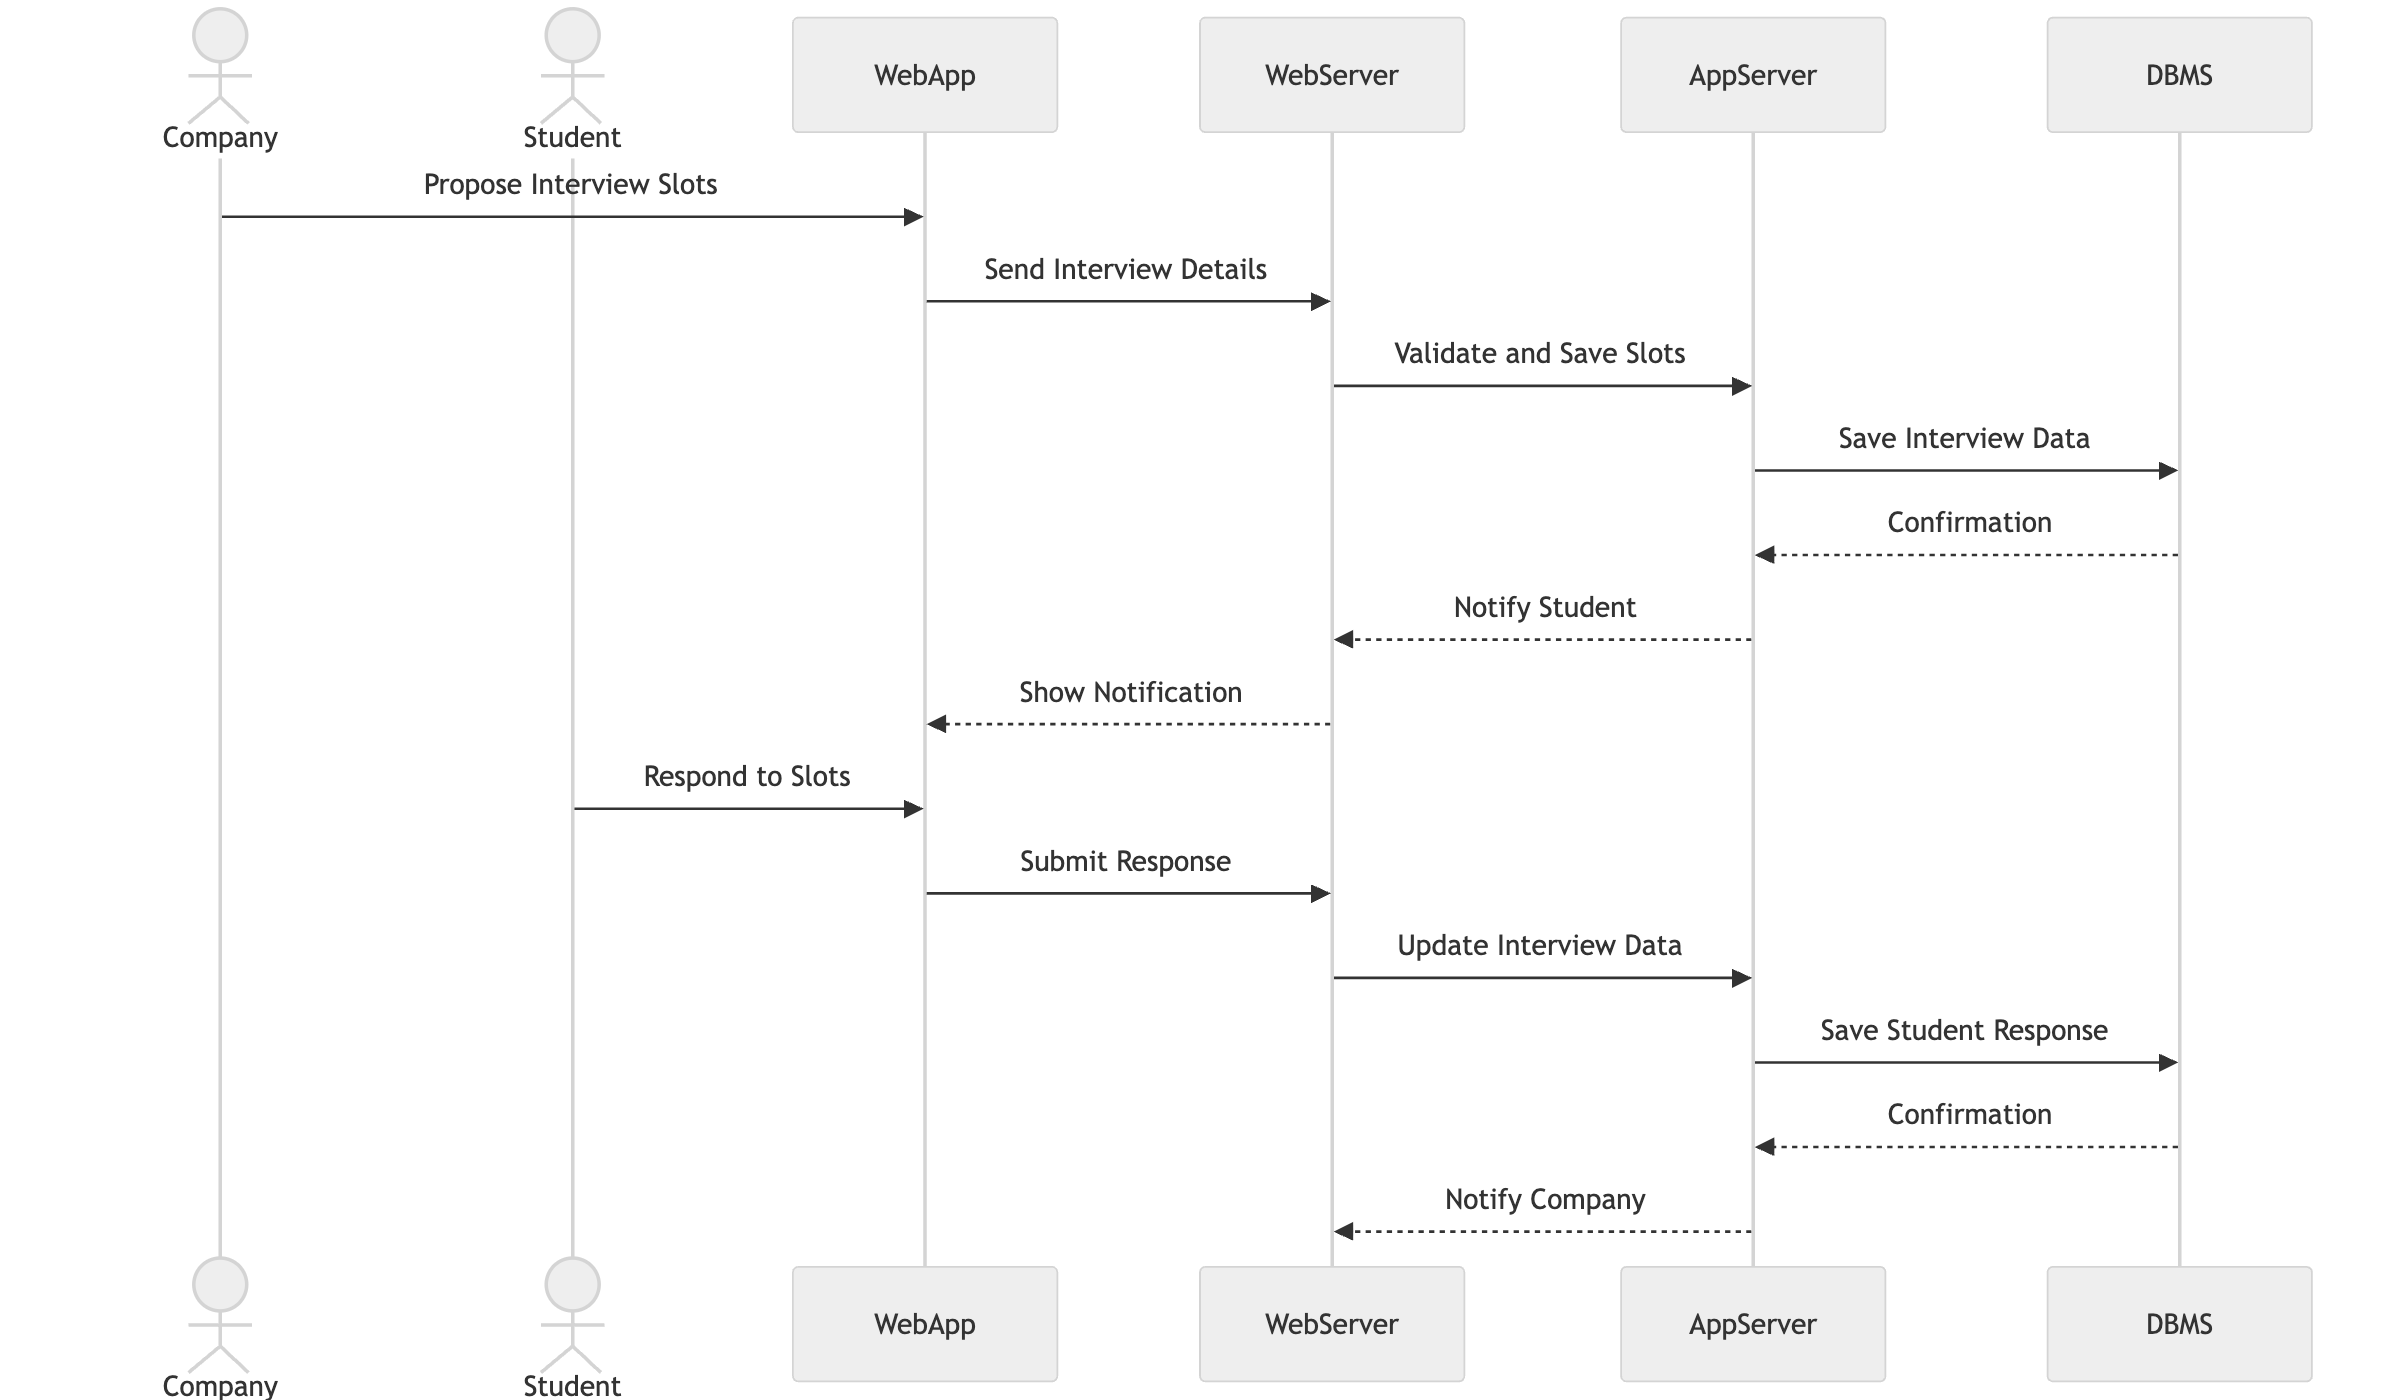
\includegraphics[width=0.82\linewidth]{JhaBhatiaSharma/imagesDD/InterviewManagementRuntime.png}
        \caption{Runtime Interview Management}
    \label{fig:interviewmanagementruntime}%
    \end{center}
\end{figure}

The interview management process streamlines scheduling and coordination between students and companies. The steps involved are:
\begin{enumerate}
    \item Employers use the WebApp to suggest interview schedules. After passing via the Web Server, the data is sent to the Application Server.
    \item The DBMS Server is used by the Interview Manager component to store the suggested timeslots in the database after verifying them.
    \item The Notification Manager and Email Server are used to inform students of the recommended timeslots.
    \item Through the WebApp, students can reply to the suggested timeslots, and the Interview Manager updates their answers in the database.
    \item The business receives notifications verifying the student's choice.
\end{enumerate}
This efficient process ensures seamless scheduling and communication for both parties.

\subsection{Complaint Handling}
\label{subsec:complaint_handling}
\begin{figure}[H]
    \begin{center}
        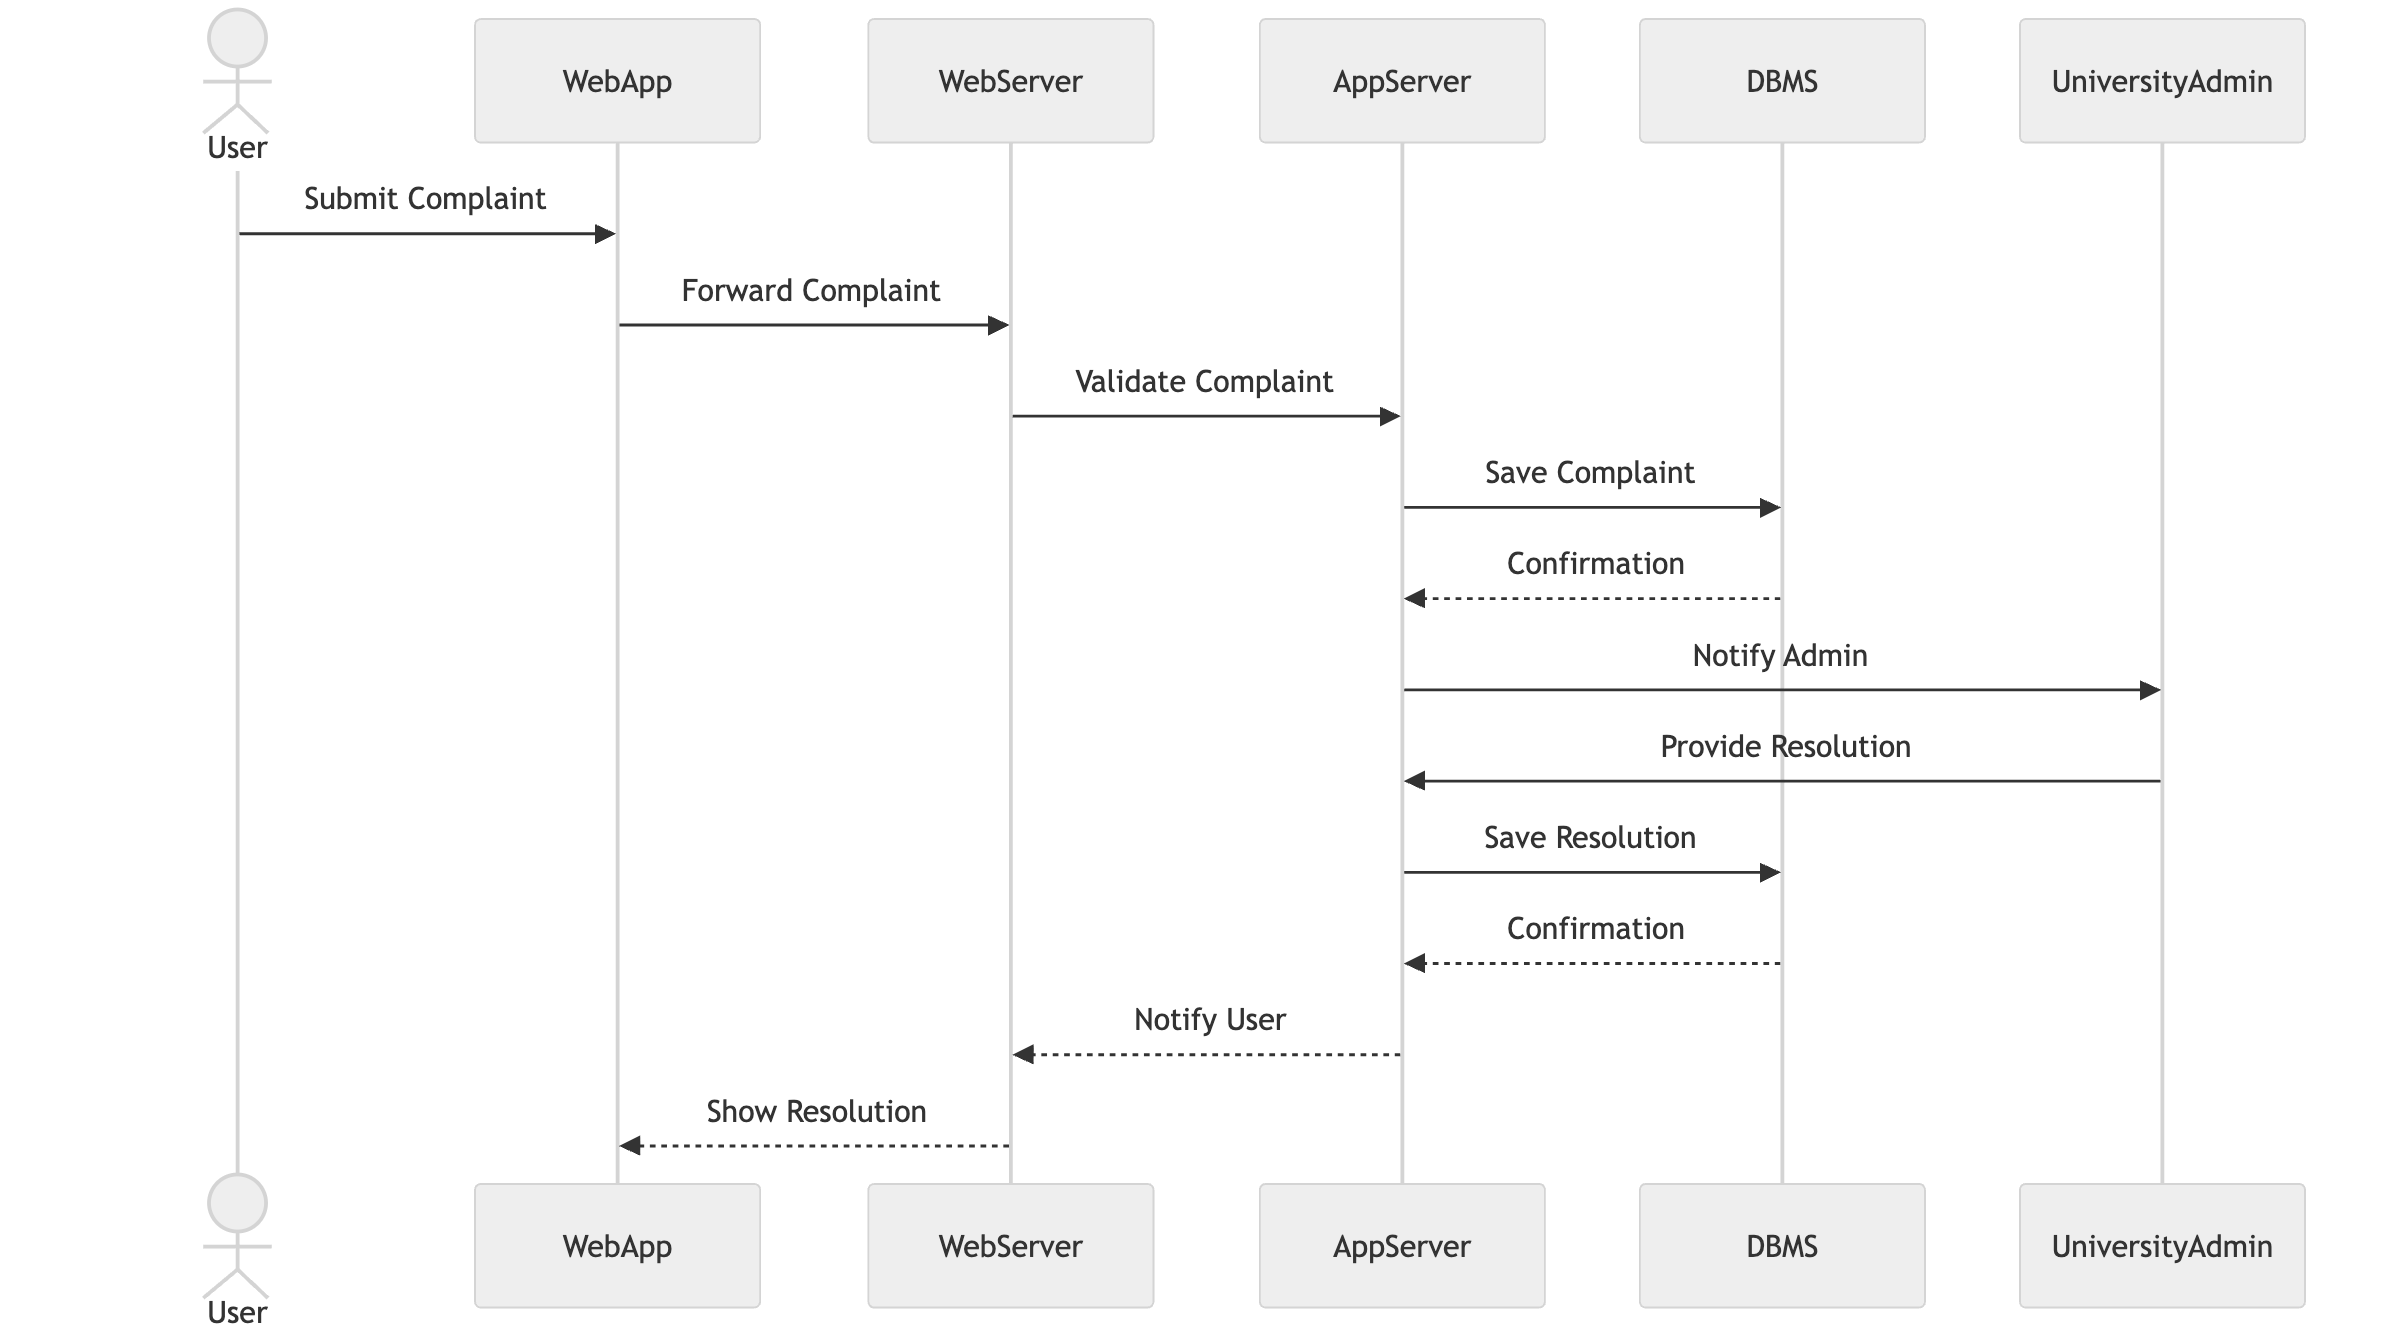
\includegraphics[width=0.82\linewidth]{JhaBhatiaSharma/imagesDD/ComplaintHandling.png}
        \caption{Complaint Handling}
        \label{fig:complainthandling}%
    \end{center}
\end{figure}
The complaint-handling process is designed to efficiently address user complaints. The steps are as follows:

\begin{enumerate}
    \item Complaints submitted by users via the WebApp are routed to the Web Server and subsequently to the Application Server.
    \item The Complaint Manager component uses the DBMS Server to store the complaint in the database after verifying it.
    \item After being informed of the complaint, the relevant university representative investigates it and offers a remedy.
    \item The user is informed of the resolution through the Email Server and Notification Manager.
    \item For future use, the resolution is noted in the database.
\end{enumerate}
This transparent process ensures that all complaints are handled promptly and efficiently.

\subsection{Profile Management}
\label{subsec:profile_management}
\begin{figure}[H]
    \begin{center}
        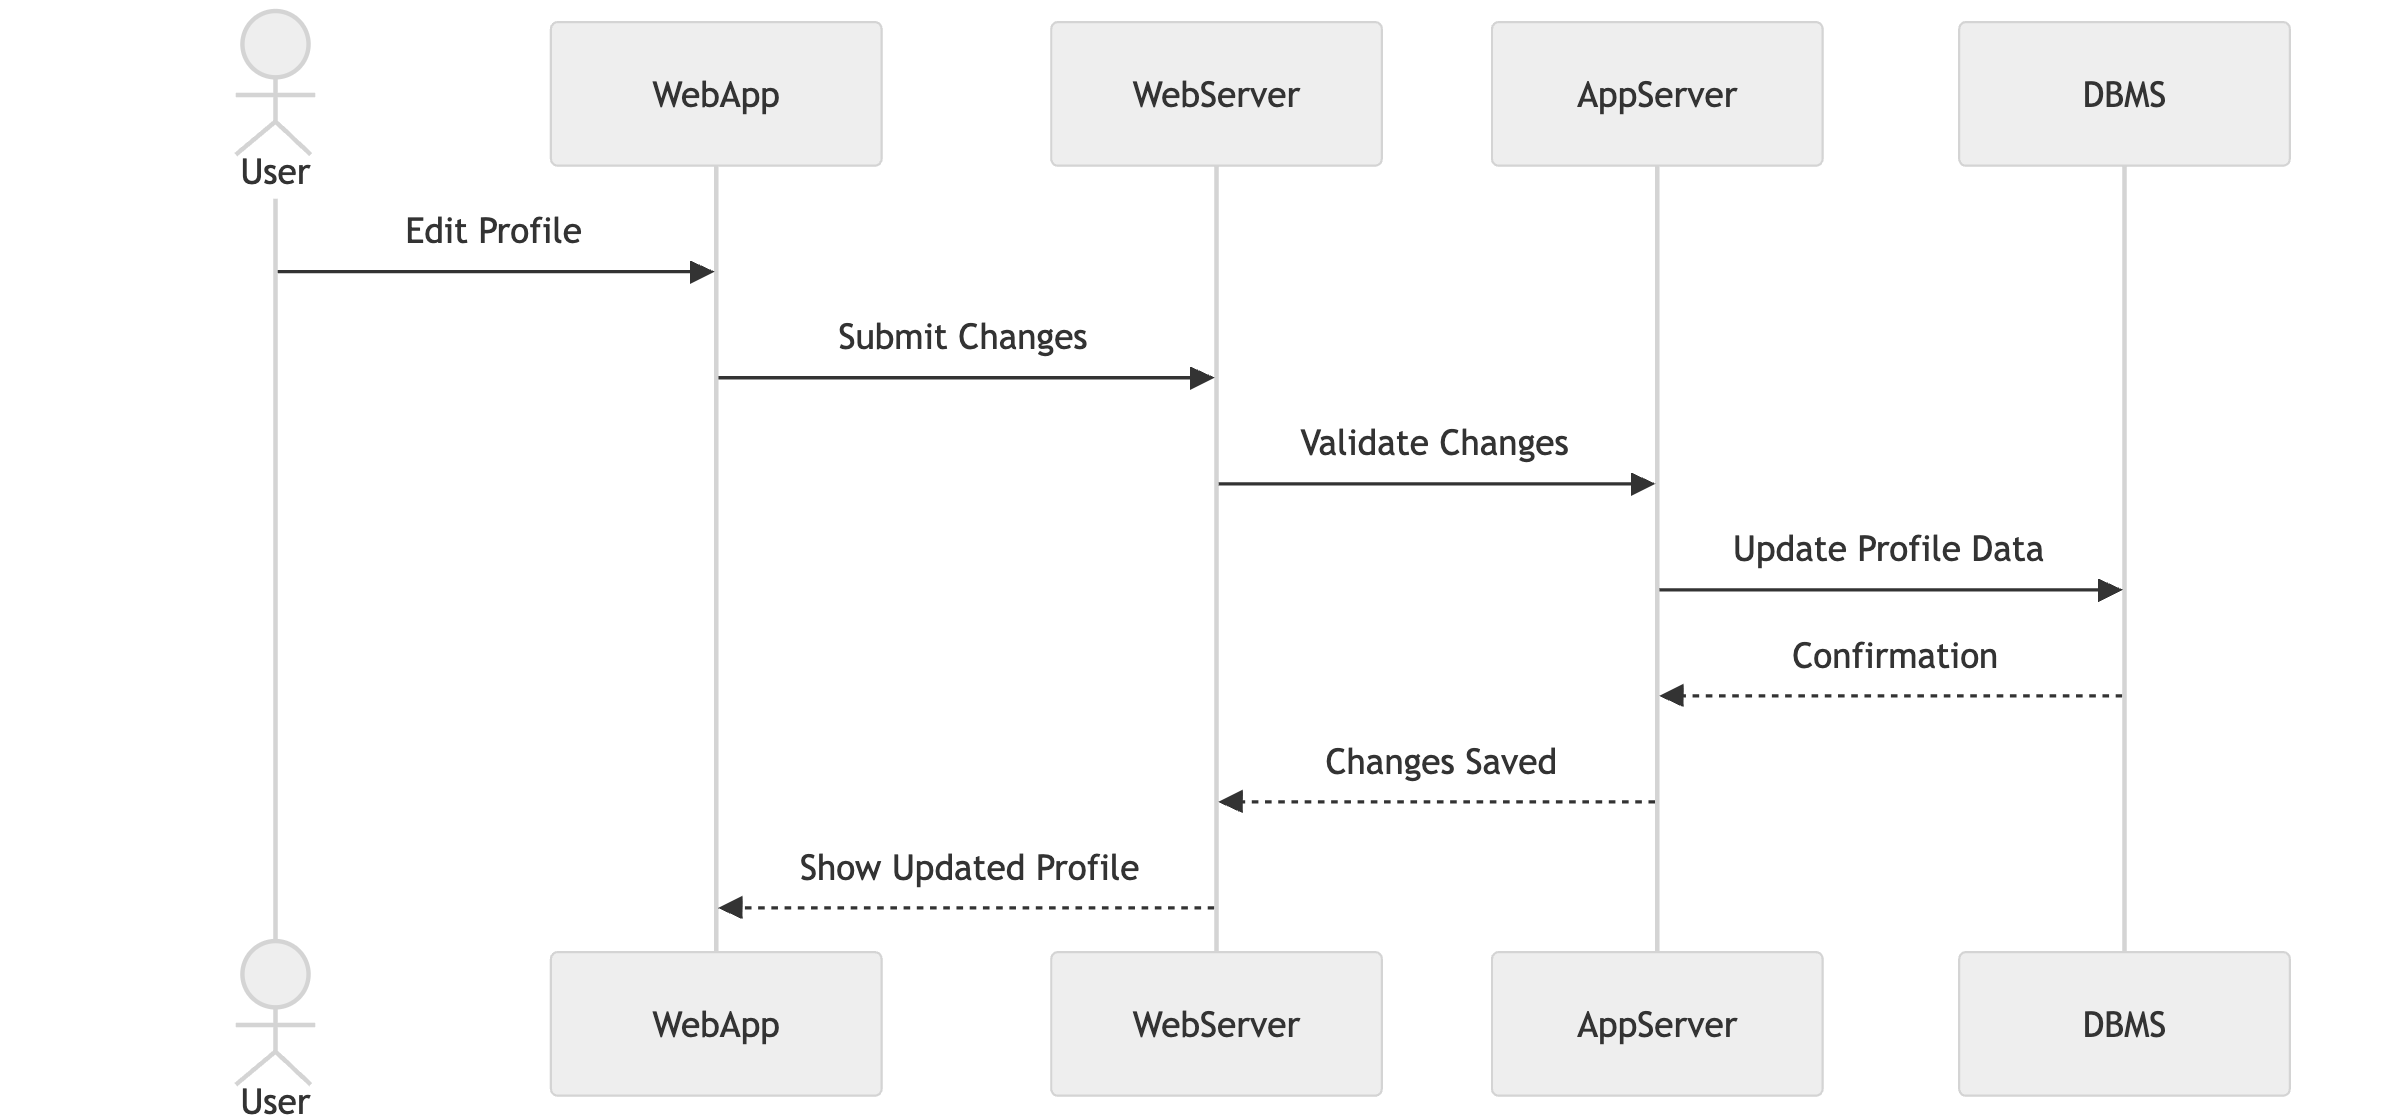
\includegraphics[width=0.82\linewidth]{JhaBhatiaSharma/imagesDD/ProfileManagement.png}
        \caption{Profile Management}
        \label{fig:profilemanagement}%
    \end{center}
\end{figure}

Profile management allows users to update and maintain their personal information. The process includes:
\begin{enumerate}
    \item Updates are started by users by inputting information including contact data, talents, and educational background on the WebApp's profile page.
    \item The Application Server receives these changes from the Web Server.
    \item In order to store the updated data in the database, the Profile Manager contacts the DBMS Server and confirms the changes.
    \item A success message is displayed to the user when the modifications have been saved.
\end{enumerate}
This feature ensures that user profiles remain up-to-date and relevant for internship matching and application processes.

\subsection{Search and Filter}
\label{subsec:search_and_filter}

\begin{figure}[H]
    \begin{center}
        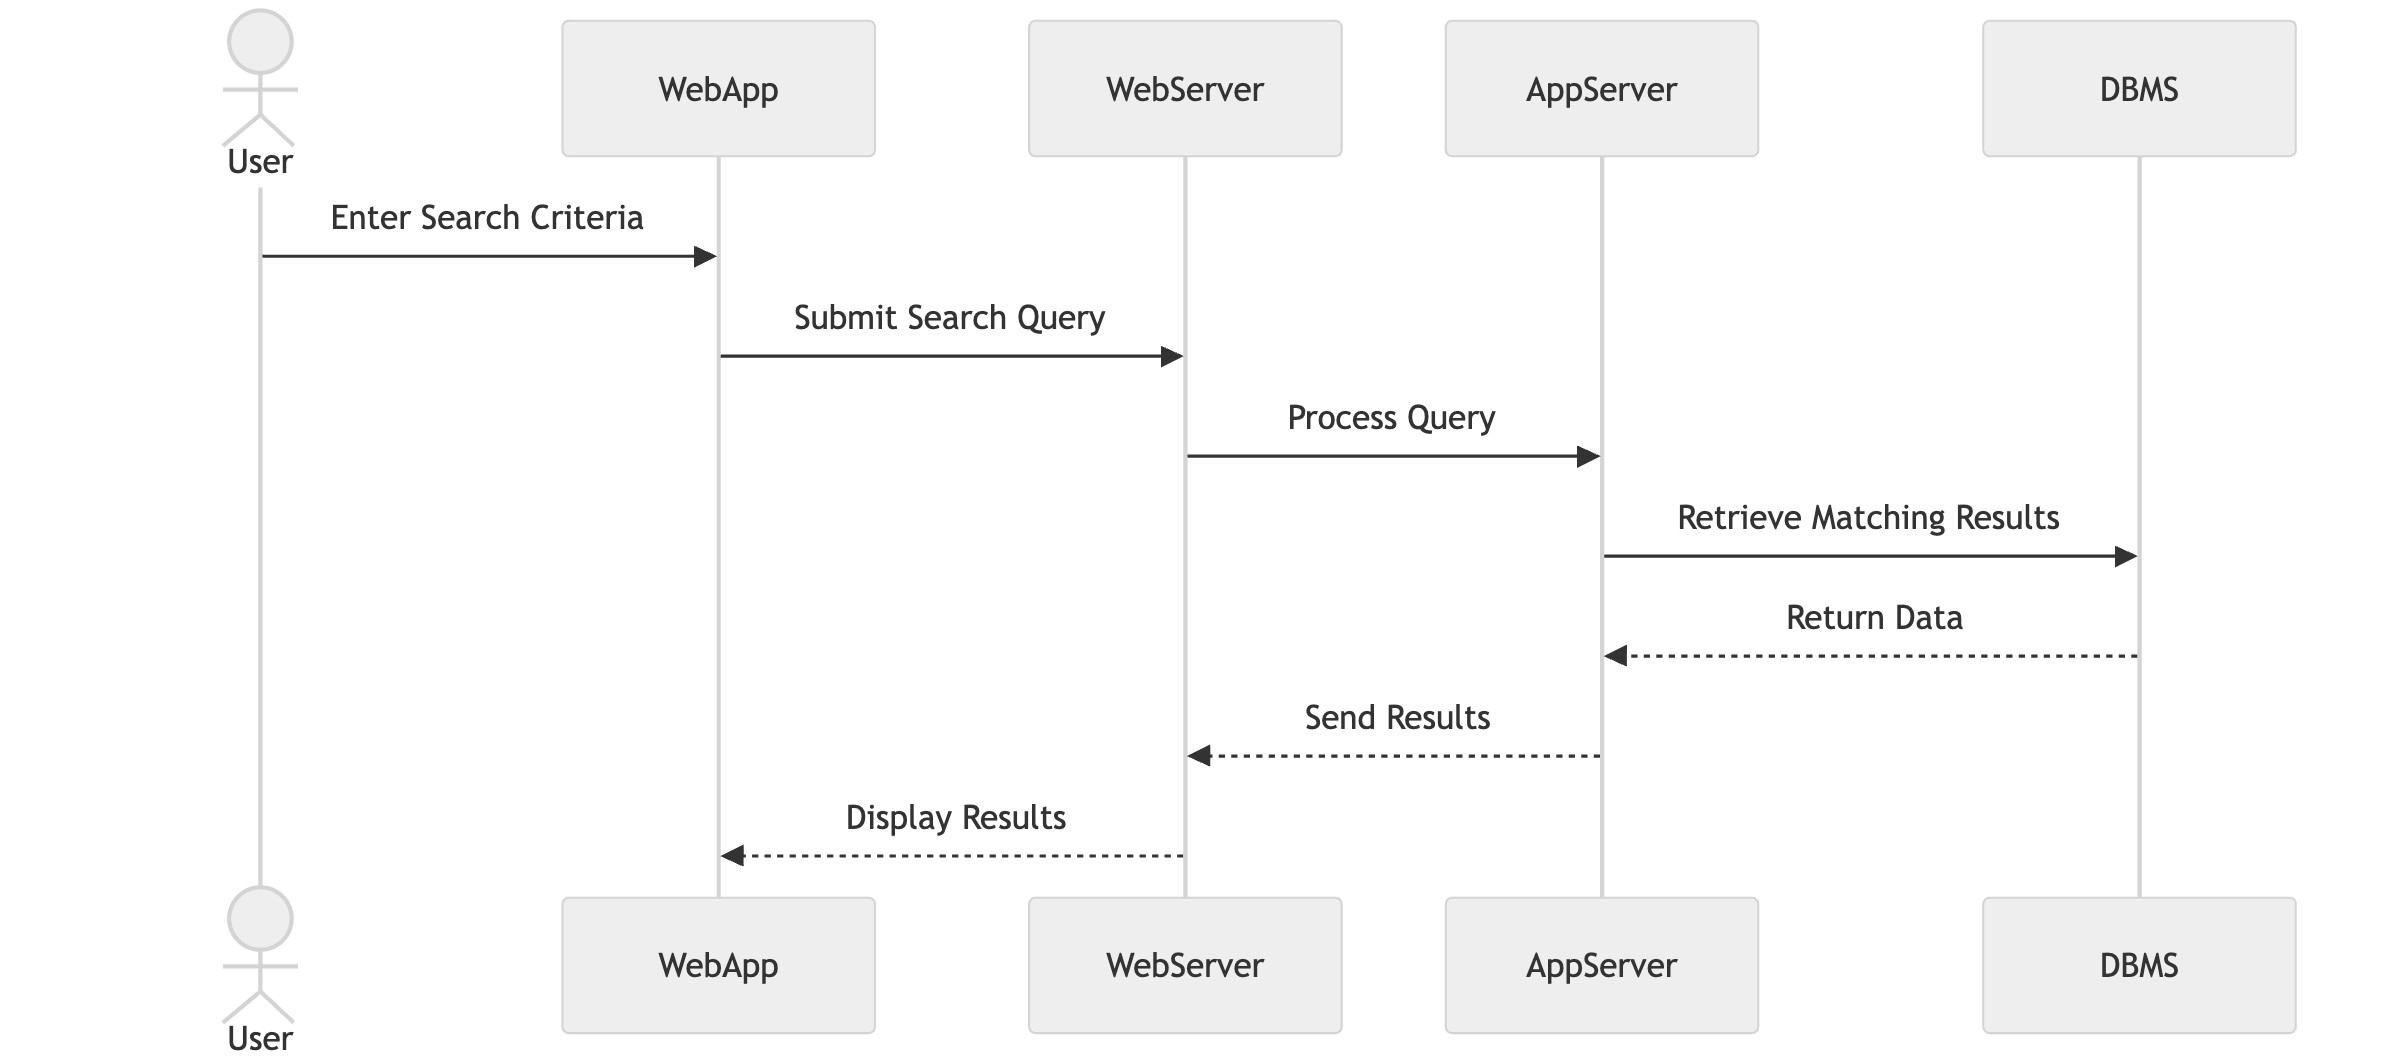
\includegraphics[width=0.82\linewidth]{JhaBhatiaSharma/imagesDD/SearchandFilter.png}
        \caption{Search and Filter}
        \label{fig:searchandfileter}%
    \end{center}
\end{figure}

The search and filter process enables users to quickly find relevant information. The workflow is as follows:
\begin{enumerate}
    \item Using the WebApp, users may search for internships by using filters like location, needed skills, and duration.
    \item These filters are sent to the Application Server by the Web Server.
    \item In order to process the query and obtain relevant results, the Search Component communicates with the DBMS Server.
    \item The WebApp receives the results from the Web Server and displays them for users to see.
\end{enumerate}
This functionality helps users efficiently navigate the platform's data and find the most relevant opportunities.

\section{Component Interfaces}
\label{subsec:component_interfaces}

\paragraph{Health Manager}
\begin{itemize}
    \item \textbf{getHealthStatus():} Verifies the health of the server and ensures it is running properly. Returns a status code and a message indicating the server status.
\end{itemize}

\paragraph{Login Manager}
\begin{itemize}
    \item \textbf{Login(String nickname, String password):} Validates user credentials and initiates a session for the user.
\end{itemize}

\paragraph{Registration Manager}
\begin{itemize}
    \item \textbf{CreateAnAccount():} Initiates the account creation process.
    \item \textbf{registerStudent(Map<String, String> studentDetails):} Registers a new student with details like name, email, and profile information.
    \item \textbf{registerRecruiter(Map<String, String> recruiterDetails):} Registers a new recruiter with details like company name, email, and profile information.
\end{itemize}

\paragraph{Internship Manager}
\begin{itemize}
    \item \textbf{addInternship(Map<String, String> internshipDetails):} enables recruiters to add a new internship following authorization validation.
    \item \textbf{deleteInternship(String internshipID):} After verifying recruiter rights, a specified internship is deleted.
    \item \textbf{fetchAllInternships(String recruiterID):} retrieves every internship that a particular recruiter has posted.
    \item \textbf{fetchInternshipById(String internshipID):} uses its ID to retrieve information on a particular internship.
\end{itemize}

\paragraph{Application Manager}
\begin{itemize}
    \item \textbf{SubmitApplication(String internshipID, String studentNickname, String resume):} gives students the opportunity to apply for a particular internship.
    \item \textbf{ViewApplications(String internshipID):} retrieves every applicant submitted for a specific internship.
    \item \textbf{UpdateApplicationStatus(String applicationID, String status):} updates a submitted application's status.
\end{itemize}

\paragraph{Interview Manager}
\begin{itemize}
    \item \textbf{ProposeInterview(String internshipID, List<Date> availableDates):} enables companies to suggest times for interviews for a particular internship.
    \item \textbf{RespondToInterview(String interviewID, String response):} gives students the option to accept or reject an invitation to an interview.
    \item \textbf{GetInterviewDetails(String interviewID):} Retrieves details about a specific interview.
\end{itemize}

\paragraph{Complaint Manager}
\begin{itemize}
    \item \textbf{SubmitComplaint(String userID, String description):} enables people to complain about a problem.
    \item \textbf{ViewComplaint(String complaintID):} brings up information on a certain complaint.
    \item \textbf{ResolveComplaint(String complaintID, String resolution):} provides an update on the complaint's status and outcome.
\end{itemize}

\paragraph{Profile Manager}
\begin{itemize}
    \item \textbf{EditProfile(String nickname, Map<String, String> updatedDetails):} Updates the user’s profile information.
    \item \textbf{ViewProfile(String nickname):} retrieves a user's profile information.
    \item \textbf{SearchProfiles(String keyword):} uses the supplied keyword to search for profiles.
\end{itemize}

\paragraph{Notification Manager}
\begin{itemize}
    \item \textbf{SendNotification(String userID, String message):} gives a user a notification.
    \item \textbf{ViewNotifications(String userID):} brings up every notification for a particular user.
\end{itemize}

\paragraph{OTP Manager}
\begin{itemize}
    \item \textbf{requestOTP(String email):} Requests an OTP for email-based authentication.
    \item \textbf{verifyOTP(String email, String otp):} confirms the OTP supplied for email authentication.
\end{itemize}

\paragraph{Token Manager}
\begin{itemize}
    \item \textbf{generateAccessToken(String email, String userType):} confirms the OTP supplied for email authentication.
\end{itemize}

\paragraph{Dashboard Manager}
\begin{itemize}
    \item \textbf{GetDashboardData(String userID):} gives the user who is logged in a summary of the dashboard.
    \item \textbf{ViewStatistics(String userID):} retrieves statistics information pertinent to the user's actions.
\end{itemize}

\section{Architectural Styles and Patterns}
\label{subsec:architectural_styles_patterns}

\subsection{Layered Architecture}
\paragraph{Front-End Layer}
\begin{itemize}
    \item Implements responsive web interfaces for three distinct user types:
    \begin{itemize}
        \item \textbf{Student Portal:} focuses on managing applications, searching for internships, and maintaining profiles.
        \item \textbf{Company Portal:} manages prospects, reviews applications, and posts internships.
        \item \textbf{Admin Portal:} offers system monitoring, complaint handling, and oversight tools.
    \end{itemize}
    \item Uses modern web technologies with responsive design principles.
    \item carries out state management and client-side validation.
\end{itemize}

\paragraph{Services Layer (Business Logic)}
\begin{itemize}
    \item \textbf{User Management Service:} manages user profiles, rights, authorization, and authentication.
    \item \textbf{Matching Engine Service:} carries out the filtering and sorting of results, processes search queries, and applies sophisticated algorithms for matching internship students.
    \item \textbf{Recommendation System:} evaluates internship requirements and student profiles to provide tailored recommendations that are updated in response to user interactions.
    \item \textbf{Interview Management Service:} oversees the scheduling of interviews, keeps track of interview status updates, and collects feedback.
\end{itemize}

\paragraph{Data Layer}
\begin{itemize}
    \item \textbf{Database Management System:} keeps organized information such as applications, internships, and user profiles. preserves relationship mappings and guarantees the consistency and integrity of data.
    \item \textbf{File Storage System:} oversees the safe uploading and downloading of files, manages the storage of documents (certificates, resumes), and applies file versioning.
\end{itemize}

\subsection{Client-Server Architecture}
\paragraph{Client Side Implementation}
\begin{itemize}
    \item uses a browser-based responsive user interface that can be adjusted to fit various screen sizes and devices.
    \item applies client-side validations and offers a consistent user experience.
\end{itemize}

\paragraph{Real-Time Updates}
\begin{itemize}
    \item Uses WebSocket connections for instant notifications.
    \item Updates UI states that preserve synchronized views without requiring a page refresh.
\end{itemize}

\paragraph{Server Side Implementation}
\begin{itemize}
    \item \textbf{RESTful API Services:} handles request/response processing, API versioning, and the implementation of defined HTTP endpoints.
    \item \textbf{Backend Processing:} Executes business logic operations, processes data transformations, and manages system state.
\end{itemize}

\subsection{Event-Driven Architecture}
\paragraph{Event Publishers}
\begin{itemize}
    \item \textbf{Application System:} activates notification workflows, creates events for status changes, and updates relevant entities.
    \item \textbf{Interview System:} creates events, notifies users of reminders, and modifies calendar integrations.
    \item \textbf{Complaint System:} Notifies the appropriate administrators, initiates escalation events, and modifies the tracking status.
\end{itemize}

\paragraph{Event Subscribers}
\begin{itemize}
    \item \textbf{Notification Service:} sends emails and alerts, handles event notifications, and modifies user dashboards.
    \item \textbf{Analytics Service:} maintains reporting metrics, creates usage statistics, and keeps track of system occurrences.
\end{itemize}

\subsection{Design Patterns}
\label{subsec:design_patterns}

\paragraph{1. Model-View-Controller (MVC)}
\begin{itemize}
    \item \textbf{Models:}
    \begin{itemize}
        \item \textbf{User Model:}
        \begin{itemize}
            \item Base user properties and behaviors.
            \item Specialized student, company, and admin classes.
            \item Data validation rules.
        \end{itemize}
        \item \textbf{Application Model:}
        \begin{itemize}
            \item Application states and transitions.
            \item Document attachments.
            \item Status tracking.
        \end{itemize}
        \item \textbf{Internship Model:}
        \begin{itemize}
            \item Position details and requirements.
            \item Application management.
            \item Scheduling information.
        \end{itemize}
    \end{itemize}
    \item \textbf{Views:}
    \begin{itemize}
        \item \textbf{User Interfaces:}
        \begin{itemize}
            \item Role-specific dashboards.
            \item Form components.
            \item Interactive elements.
        \end{itemize}
        \item \textbf{Data Presentation:}
        \begin{itemize}
            \item Lists and tables.
            \item Search results.
            \item Statistical reports.
        \end{itemize}
    \end{itemize}
    \item \textbf{Controllers:}
    \begin{itemize}
        \item \textbf{Authentication Controller:}
        \begin{itemize}
            \item Login/logout handling.
            \item Session management.
            \item Access control.
        \end{itemize}
        \item \textbf{Application Controller:}
        \begin{itemize}
            \item Process submissions.
            \item Status updates.
            \item Document handling.
        \end{itemize}
    \end{itemize}
\end{itemize}

\paragraph{2. Observer Pattern}
\begin{itemize}
    \item \textbf{Subject Components:}
    \begin{itemize}
        \item \textbf{Internship Posting System:}
        \begin{itemize}
            \item Notifies matched students.
            \item Updates search results.
            \item Triggers recommendations.
        \end{itemize}
        \item \textbf{Application Processing:}
        \begin{itemize}
            \item Updates stakeholders.
            \item Triggers next steps.
            \item Maintains status logs.
        \end{itemize}
    \end{itemize}
    \item \textbf{Observer Components:}
    \begin{itemize}
        \item \textbf{Student Notifications:}
        \begin{itemize}
            \item New matching internships.
            \item Application updates.
            \item Interview schedules.
        \end{itemize}
        \item \textbf{Company Notifications:}
        \begin{itemize}
            \item New applications.
            \item Interview confirmations.
            \item Status changes.
        \end{itemize}
    \end{itemize}
\end{itemize}

\paragraph{3. Factory Pattern}
\begin{itemize}
    \item \textbf{User Factory:}
    \begin{itemize}
        \item Creates appropriate user types.
        \item Initializes role-specific properties.
        \item Sets up required relationships.
    \end{itemize}
    \item \textbf{Document Factory:}
    \begin{itemize}
        \item Generates different document types.
        \item Handles format conversions.
        \item Creates appropriate storage entries.
    \end{itemize}
\end{itemize}

\paragraph{4. State Pattern}
\begin{itemize}
    \item \textbf{Application States:}
    \begin{itemize}
        \item Submitted.
        \item Under Review.
        \item Interview Scheduled.
        \item Accepted/Rejected.
        \item Completed.
    \end{itemize}
    \item \textbf{Complaint States:}
    \begin{itemize}
        \item Filed.
        \item Under Investigation.
        \item Resolved.
        \item Closed.
        \item Escalated.
    \end{itemize}
\end{itemize}

\paragraph{5. Strategy Pattern}
\begin{itemize}
    \item \textbf{Matching Strategies:}
    \begin{itemize}
        \item Skills-based matching.
        \item Location-based matching.
        \item Experience-level matching.
        \item Industry-specific matching.
    \end{itemize}
    \item \textbf{Search Strategies:}
    \begin{itemize}
        \item Keyword search.
        \item Filter-based search.
        \item Category-based search.
        \item Combined search approaches.
    \end{itemize}
\end{itemize}

\paragraph{Benefits of Implementing Design Patterns:}
\begin{itemize}
    \item Clear separation of concerns.
    \item Maintainable and scalable codebase.
    \item Robust error handling.
    \item Secure data management.
    \item Efficient performance.
    \item Real-time responsiveness.
    \item Consistent user experience.
\end{itemize}

\section{Other Design Decisions}
\label{sec:other_design_decisions}

\subsection{Availability}
\label{subsec:availability}
\begin{itemize}
    \item Redundant systems guarantee uninterrupted, 24/7 platform operation.
    \item During interruptions, a failover mechanism allows for automatic shift to backup systems.
    \item Data integrity is guaranteed by error handling procedures.
    \item System recovery procedures after failures.
    \item Transaction integrity for important procedures such as scheduling interviews and submitting applications.
\end{itemize}

\subsection{Scalability}
\label{subsec:scalability}
\begin{itemize}
    \item Front-end layer scalability for multiple user portals (Student, Company, Admin).
    \item Services layer that can scale independently based on demand:
    \begin{itemize}
        \item User Management Service.
        \item Matching Engine.
        \item Recommendation System.
        \item Interview Management Service.
    \end{itemize}
    \item Systems for databases and storage that can handle increasing amounts of data.
    \item API-first approach enabling future mobile app development.
\end{itemize}

\subsection{Security}
\label{subsec:security}
\begin{itemize}
    \item Robust authentication systems for user verification.
    \item authorization for sensitive operations based on roles.
    \item End-to-end data encryption.
    \item GDPR compliance measures.
    \item Secure document storage and handling.
    \item routine security monitoring and audits.
\end{itemize}

\subsection{Notification Handling}
\label{subsec:notification_handling}
\begin{itemize}
    \item Notifications in real time when the status of an application changes.
    \item Interview scheduling alerts.
    \item Complaint status updates.
    \item Notifications about important occurrences via email.
    \item Integration of a calendar to schedule interviews.
    \item Platform-wide announcements capability.
\end{itemize}

\subsection{Document Management}
\label{subsec:document_management}
\begin{itemize}
    \item Certificates, formal documents, and resumes should all be stored securely.
    \item Version control for user documents.
    \item Document validation and verification.
    \item Format standardization.
    \item Access control based on user roles.
    \item Automated capacity for processing documents.
\end{itemize}

\subsection{Data Persistence}
\label{subsec:data_persistence}
\begin{itemize}
    \item Centralized database for core functionality:
    \begin{itemize}
        \item User profiles.
        \item Internship listings.
        \item Applications.
        \item Interview records.
        \item Complaints.
    \end{itemize}
    \item File storage system for documents.
    \item Data backup and recovery systems.
    \item Audit logging for critical operations.
    \item Data retention policies compliance.
\end{itemize}

\subsection{Performance Optimization}
\label{subsec:performance_optimization}
\begin{itemize}
    \item Page load optimization (\textless 5 seconds).
    \item Search results delivery (\textless 2 seconds).
    \item File upload handling (\textless 10 seconds for 10MB).
    \item Real-time updates (\textless 1 second).
    \item Concurrent user support (up to 50 users).
    \item Database transaction optimization (10 transactions per second).
\end{itemize}

\paragraph{Alignment with Platform Goals:}
These design decisions align with the platform's core requirements while ensuring:
\begin{itemize}
    \item Reliable service delivery.
    \item Secure data handling.
    \item Efficient performance.
    \item User satisfaction.
    \item System maintainability.
    \item Regulatory compliance.
    \item Future scalability.
\end{itemize}
